%===================================== CHAP  =================================
%===================================== CHAP 7 =================================

The results of this work are presented in two sections. The first section is the results of the sample preparation including polishing, lithography, contact deposition, and oven annealing of the samples. The second section contains the results on of electrical measurements on fibers, and comparisons of coatings on SiGe and Si Fibers.

\section{Sample Preparation}

\subsection{Polishing}
%surface quality
%EBSD

\subsubsection{3d profilometer image of surface roughness}


\begin{figure}[h]
 %h here H requires float, exactly here, h! overide latex
\centering
\begin{subfigure}{\textwidth}
  \centering
  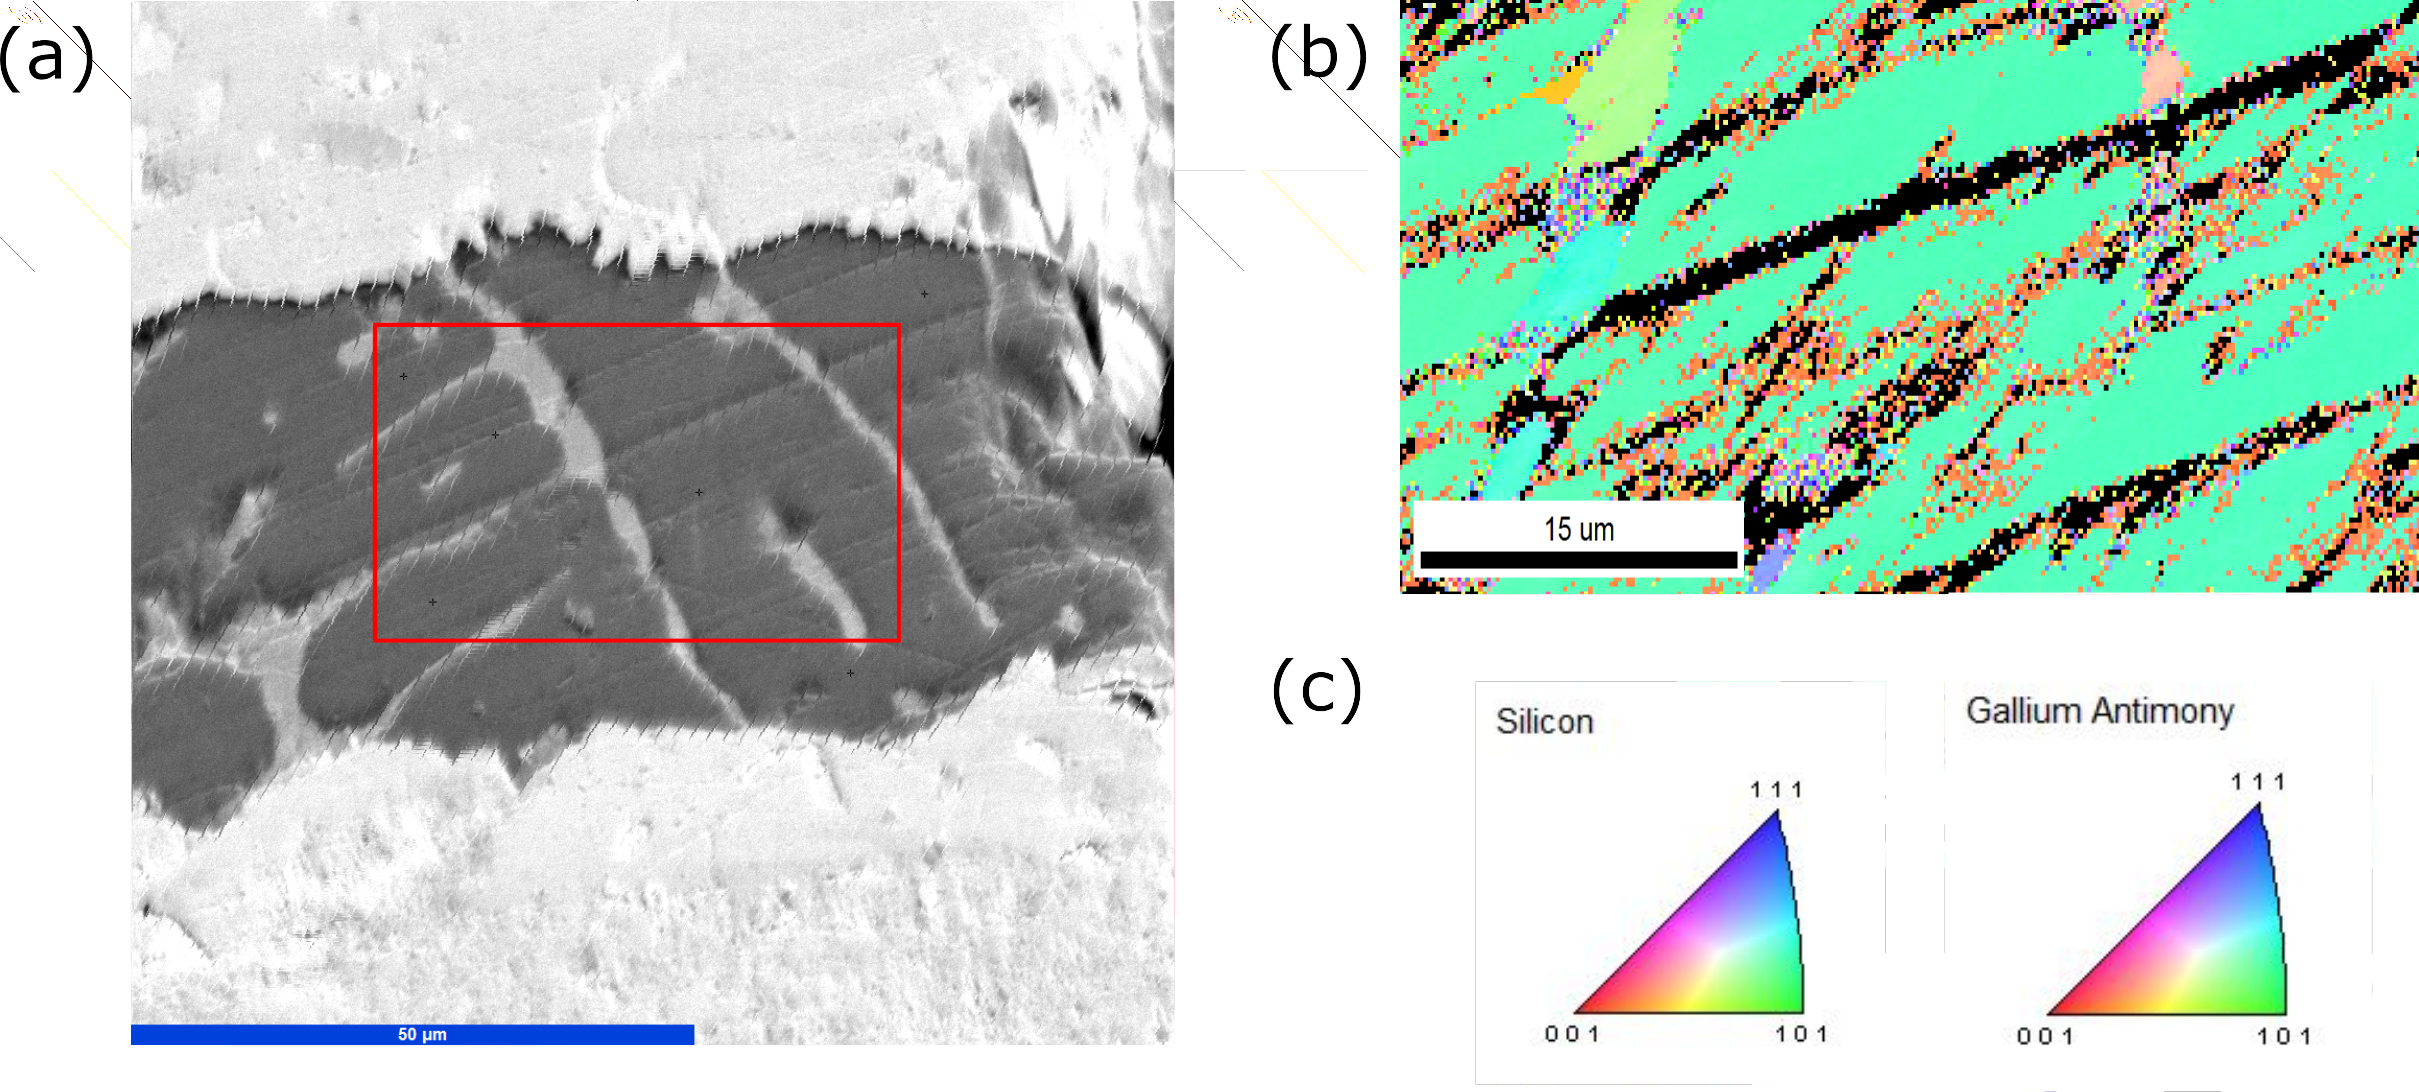
\includegraphics[width=\linewidth]{fig/Results/gasb.png}
  %\caption{1a}
  \label{fig:sfig1}
\end{subfigure}% %blank line makes figures vertical

\begin{subfigure}{\textwidth}
  \centering
  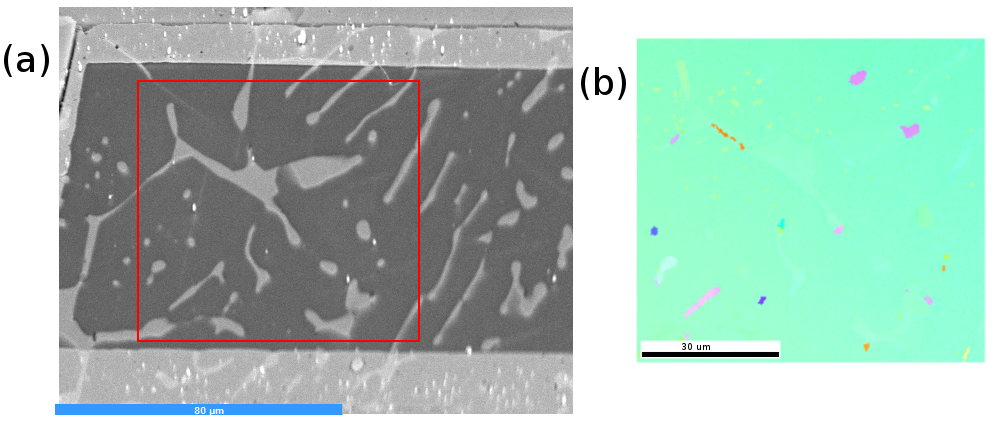
\includegraphics[width=\linewidth]{fig/ebsd_machinepolish.png}
  %\caption{1a}
  \label{fig:sfig2}
\end{subfigure}% %blank line makes figures vertical

\caption{EBSD results of GaSb fiber after polish by hand(top) and machine(bottom). EBSD imaging and hand polishing performed by Seunghan Song}
\label{fig:ebsd}
\end{figure}

\FloatBarrier
\subsection{Stress and Cracking}
Discussion of cracking and possible changes with oven annealing

\begin{figure}[h]
 %h here H requires float, exactly here, h! overide latex
\centering
\begin{subfigure}{.7\textwidth}
  \centering
  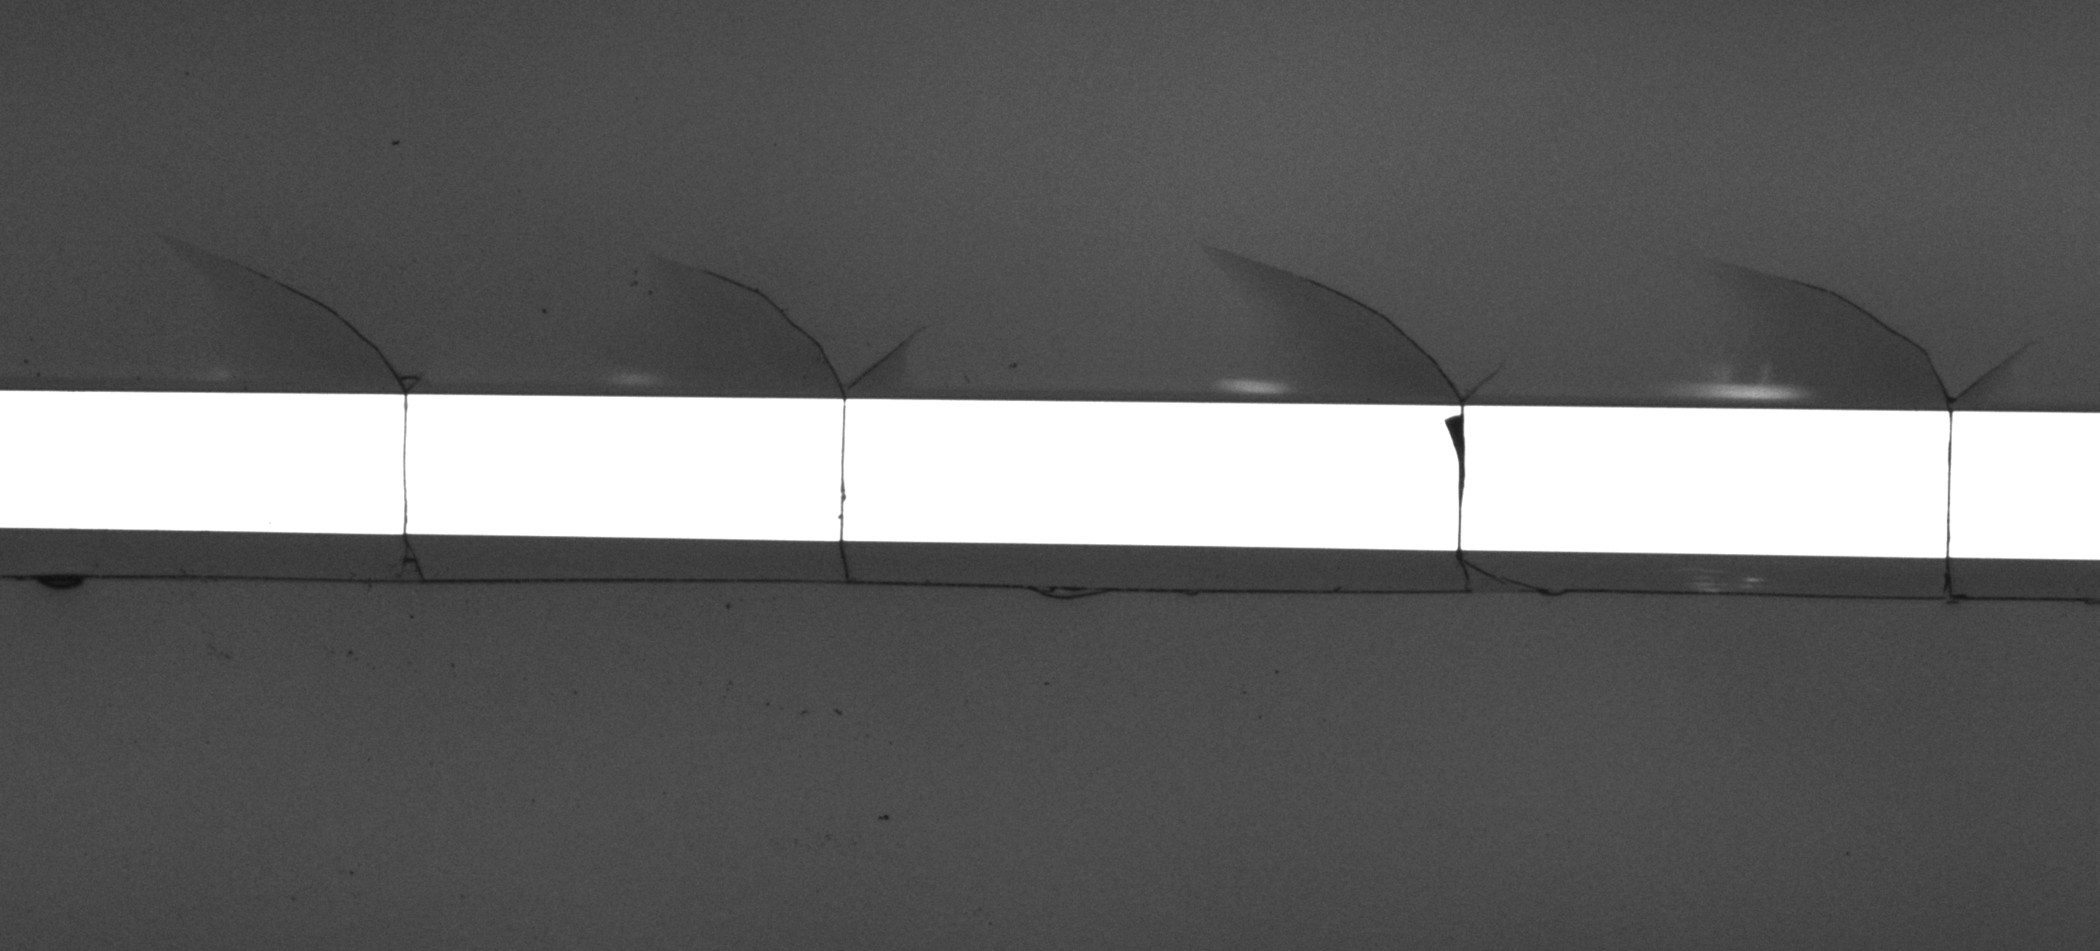
\includegraphics[width=\linewidth]{fig/polishing/Siedit.jpg}
  %\caption{1a}
  \label{fig:sfig1}
\end{subfigure}% %blank line makes figures vertical

\begin{subfigure}{.7\textwidth}
  \centering
  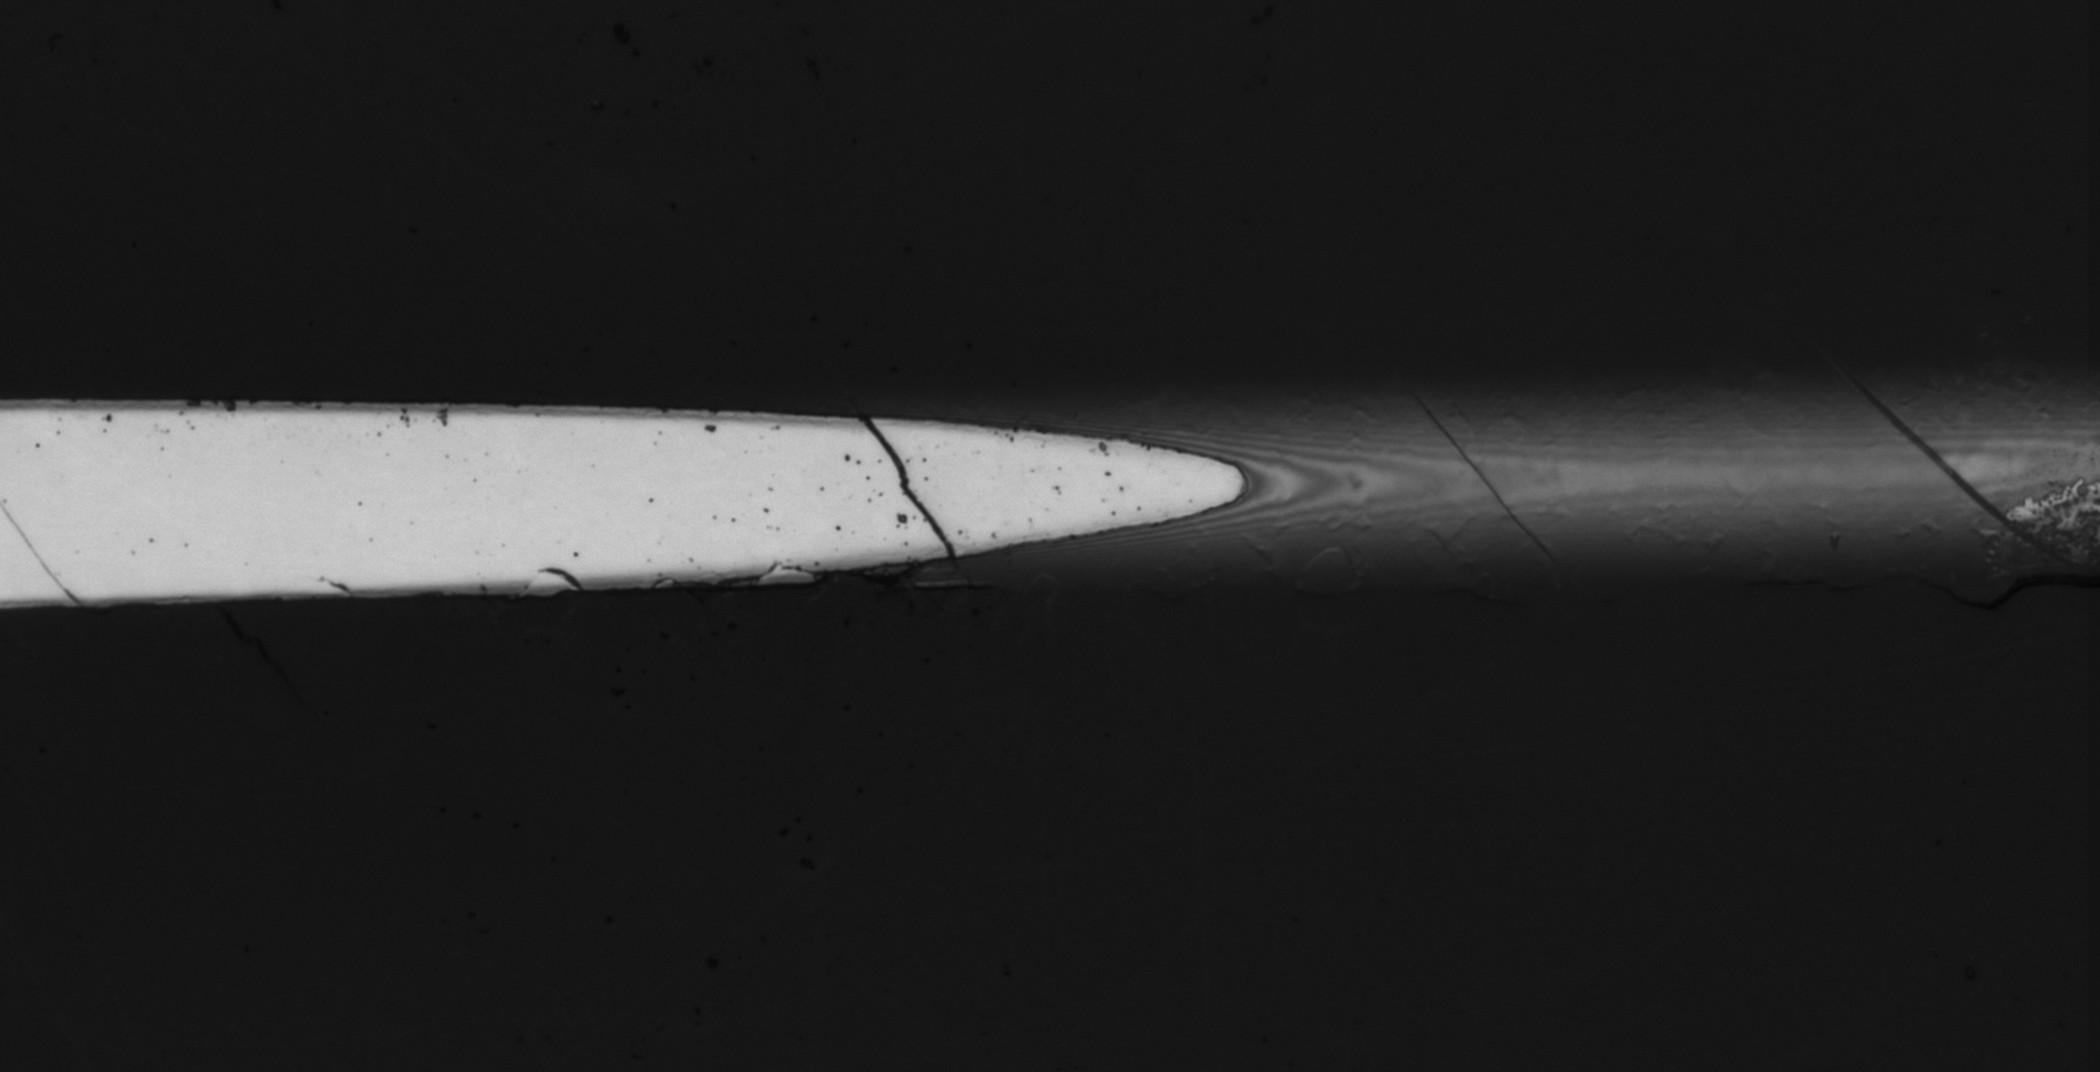
\includegraphics[width=\linewidth]{fig/polishing/SiGe.jpg}
  %\caption{1a}
  \label{fig:sfig2}
\end{subfigure}% %blank line makes figures vertical

\begin{subfigure}{.7\textwidth}
  \centering
  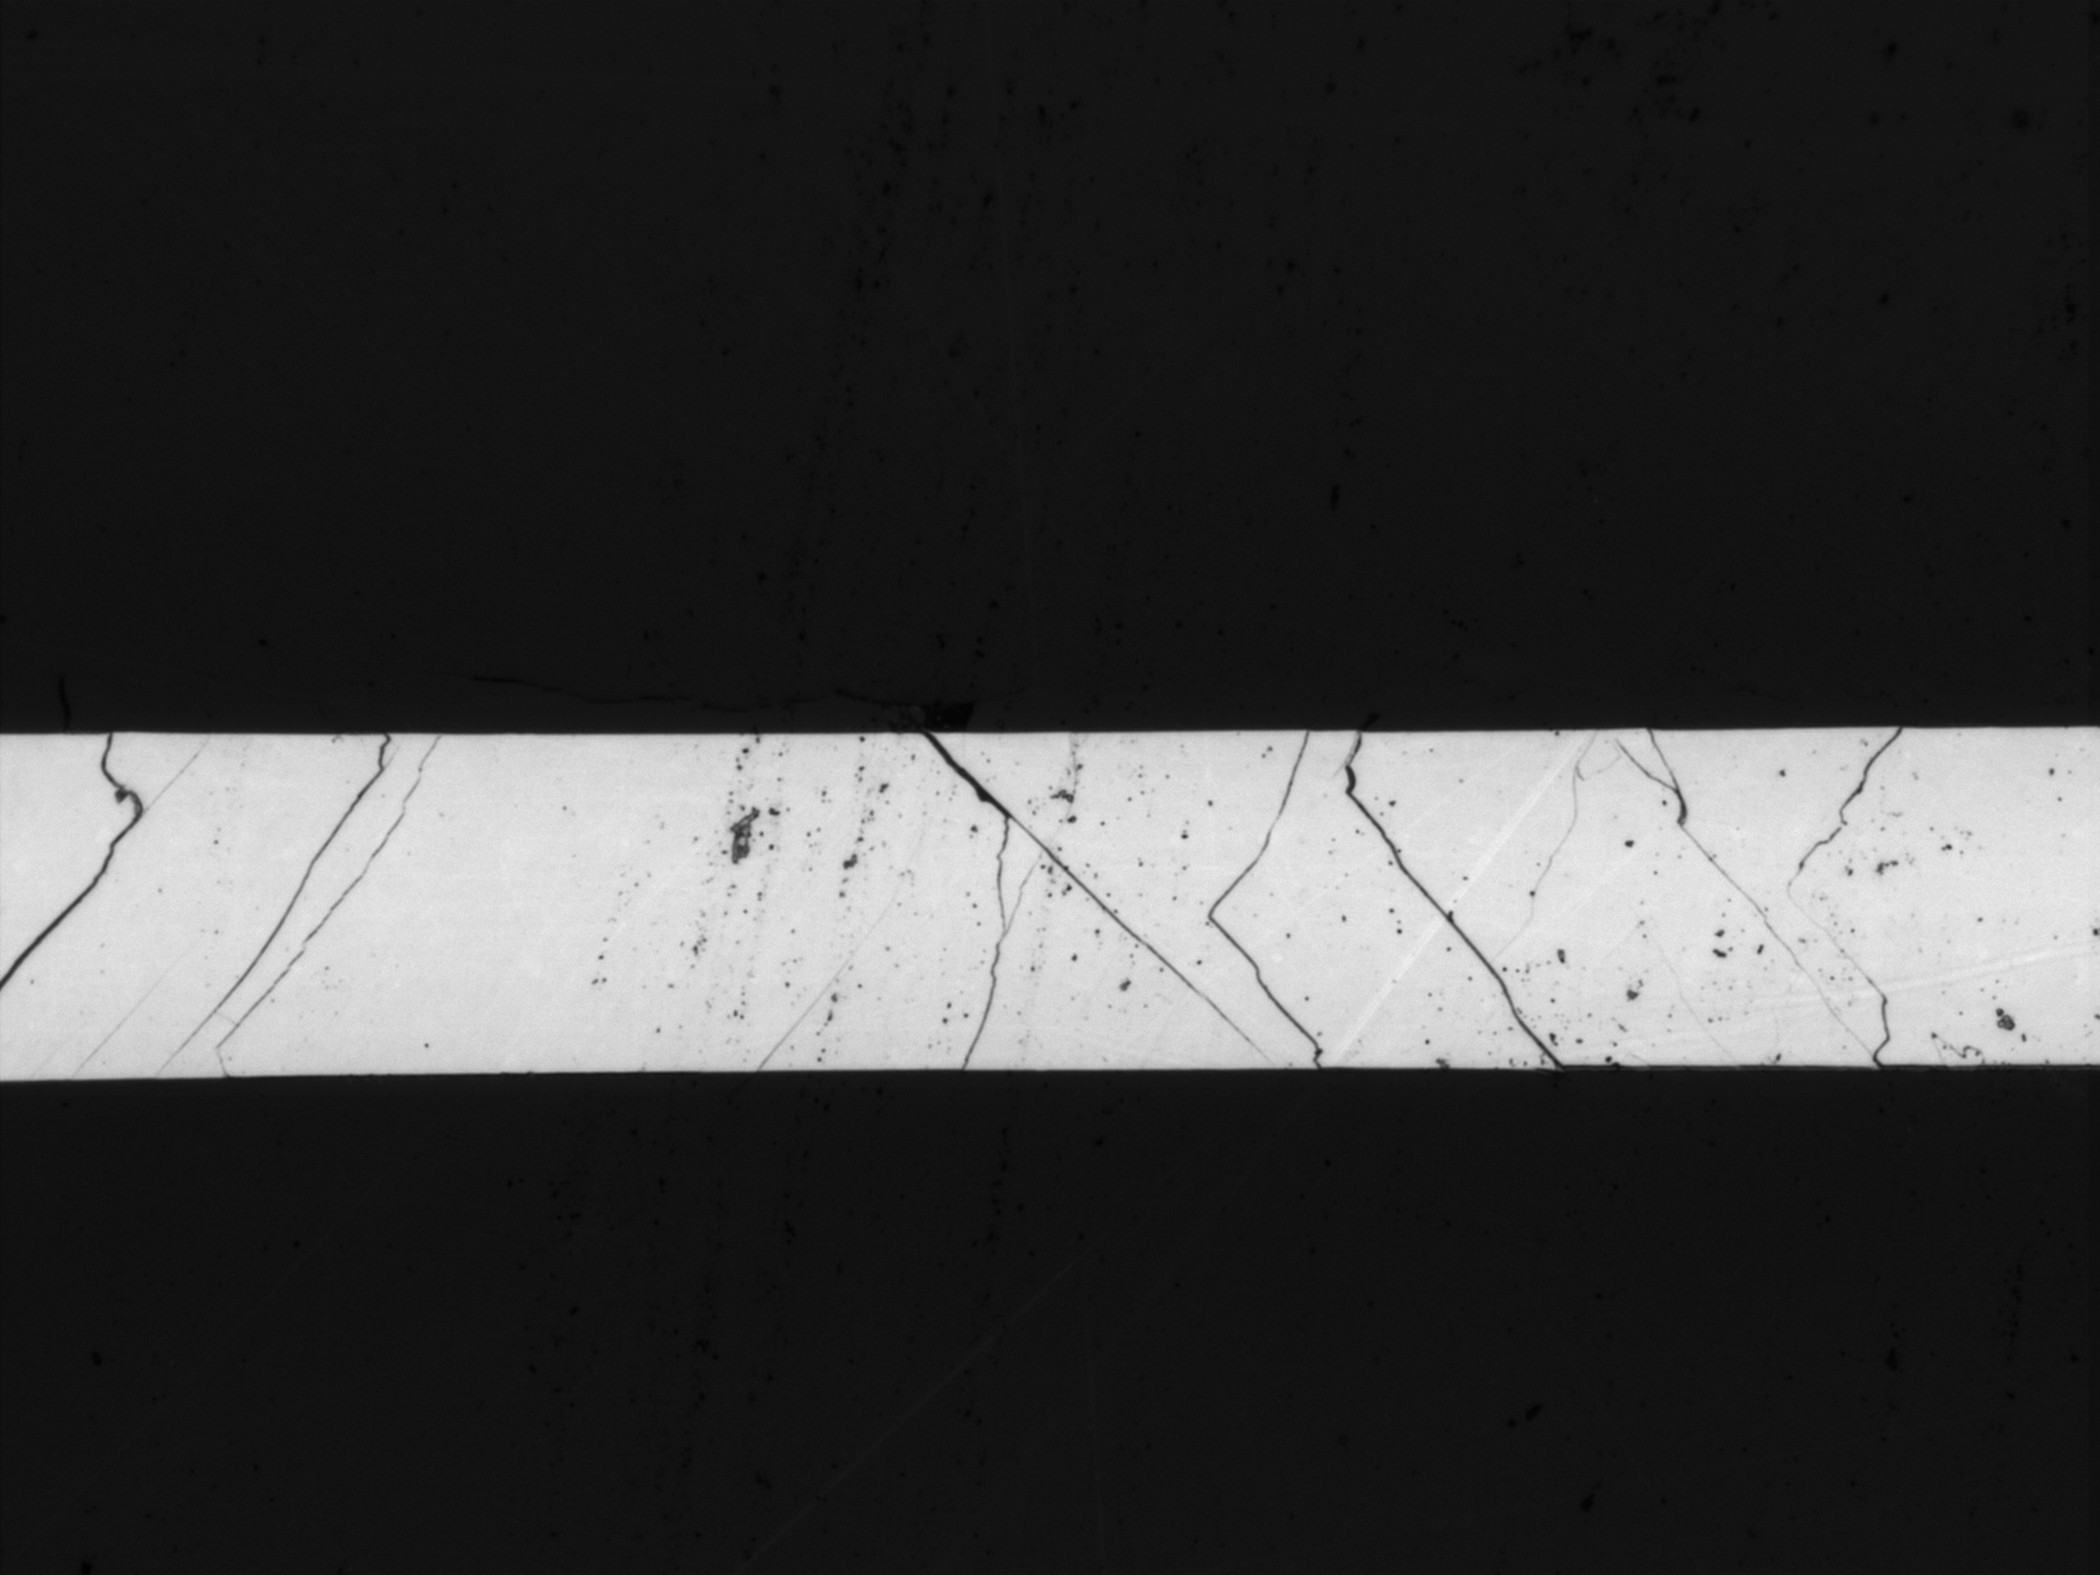
\includegraphics[width=\linewidth]{fig/polishing/SiGe2.jpg}
  %\caption{1b}
  \label{fig:sfig3}
\end{subfigure}
\caption{}
\label{fig:si_sige}
\end{figure}


\begin{figure}[h]
 %h here H requires float, exactly here, h! overide latex
\centering
\begin{subfigure}{.7\textwidth}
  \centering
  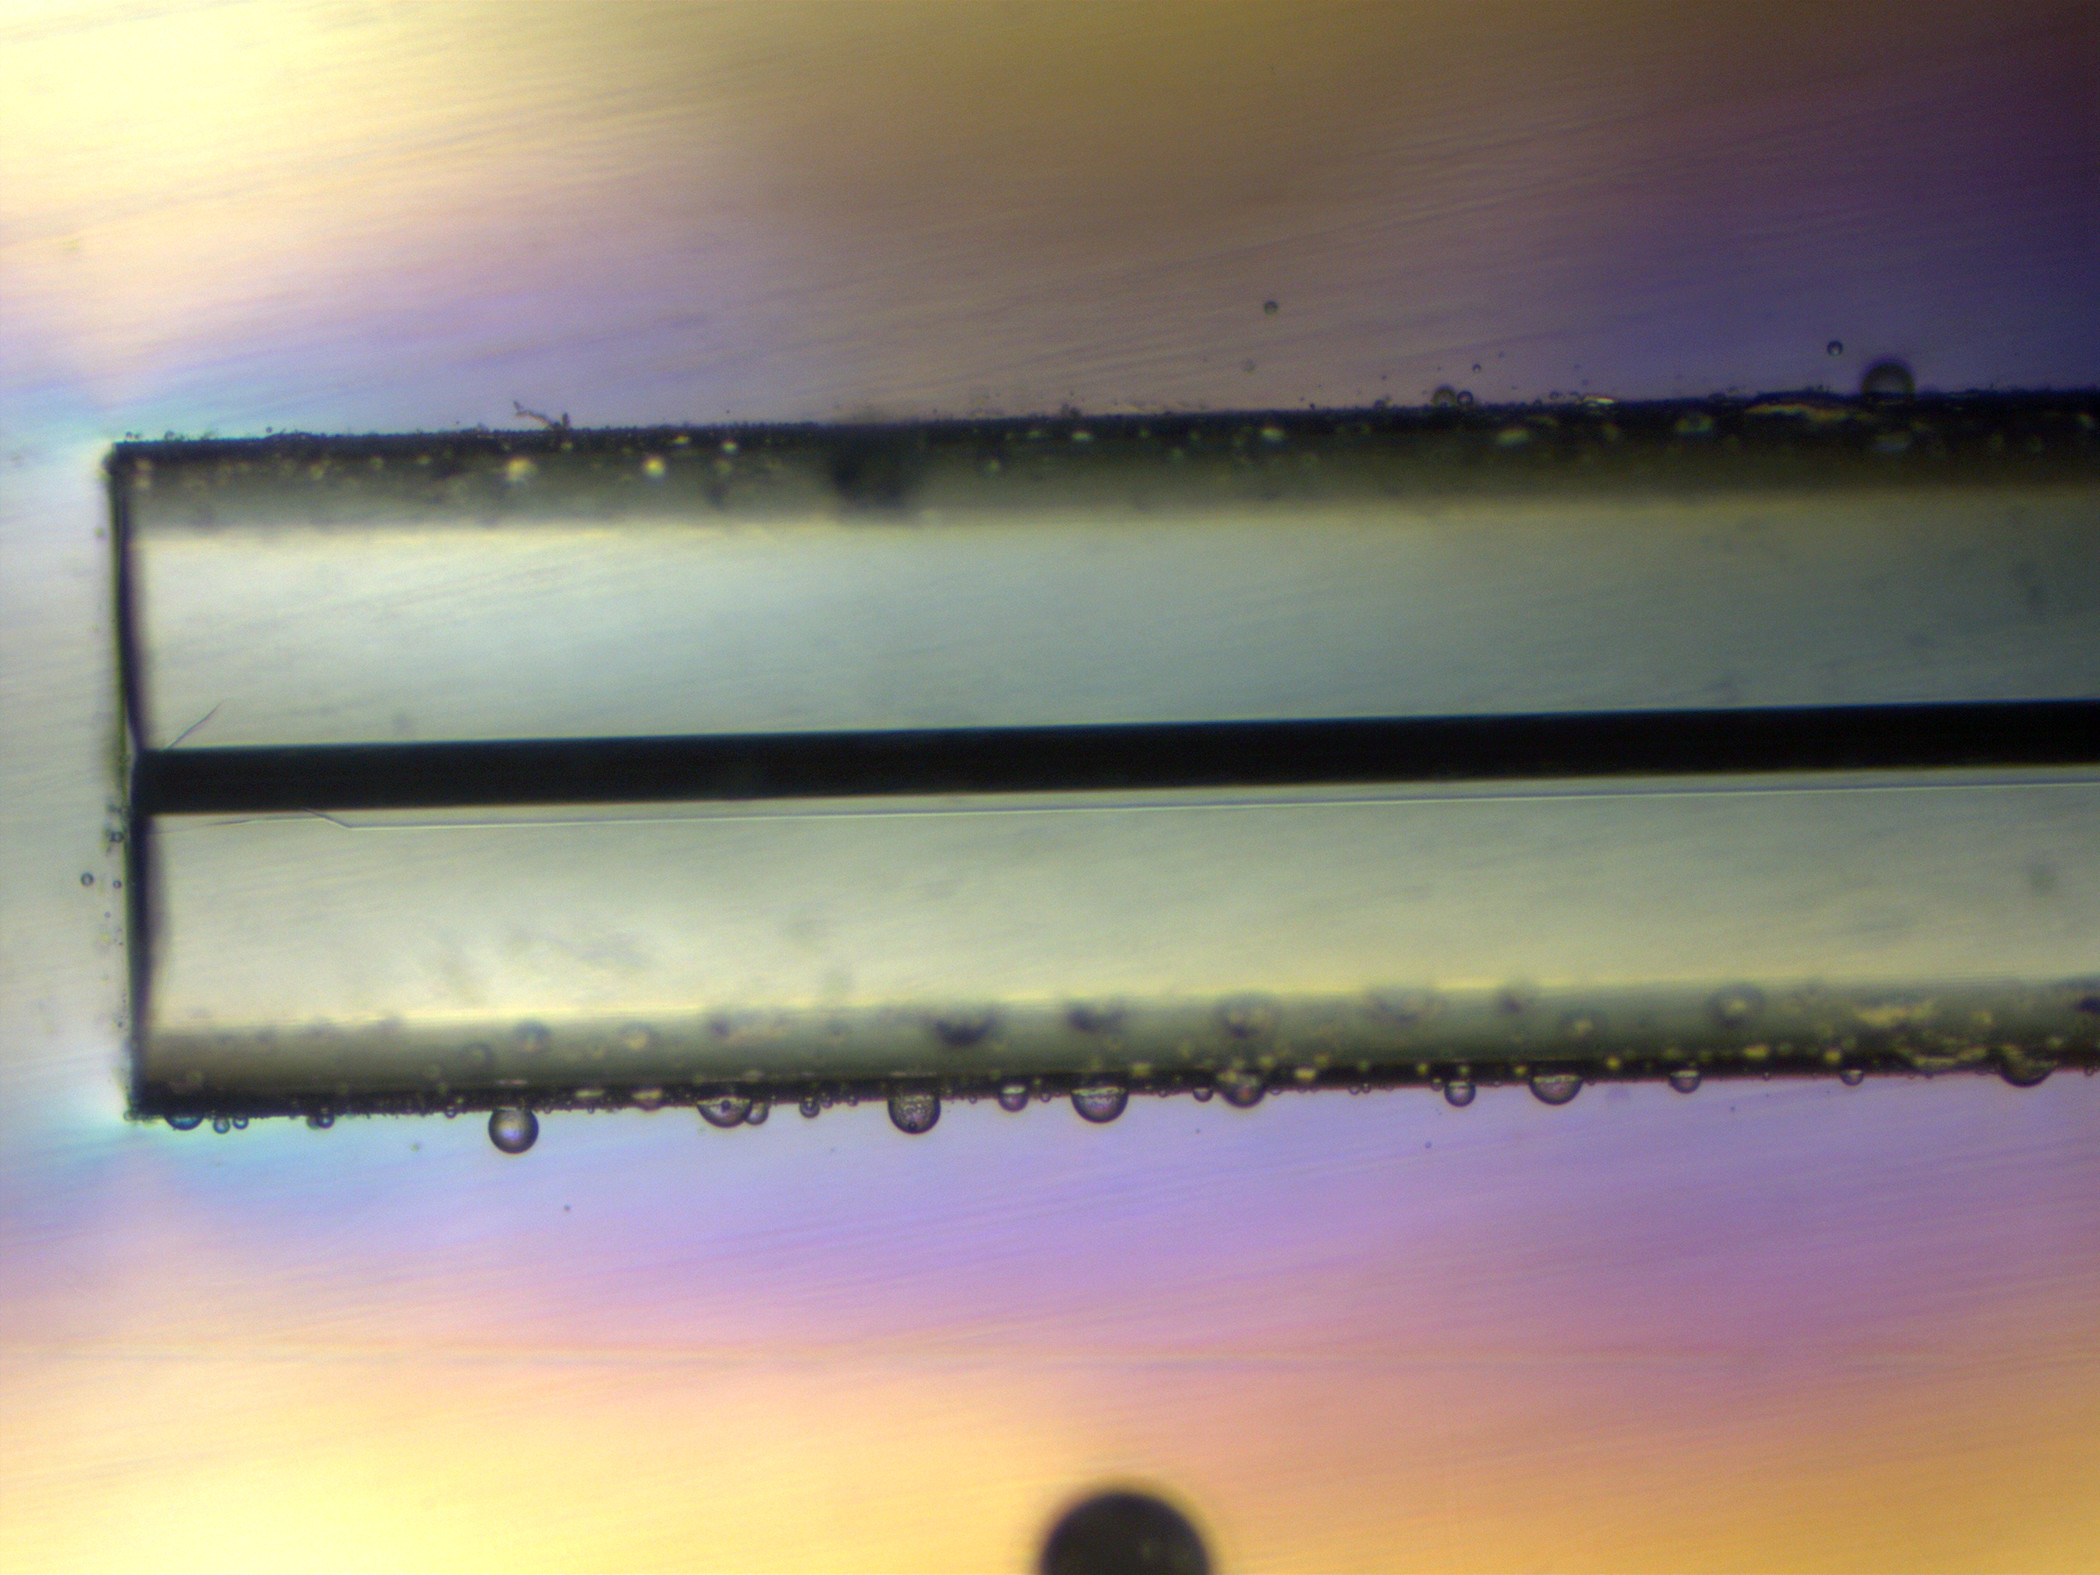
\includegraphics[width=\linewidth]{fig/polishing/parallelcrack.jpg}
  %\caption{1a}
  \label{fig:sfig1}
\end{subfigure}% %blank line makes figures vertical

\begin{subfigure}{.7\textwidth}
  \centering
  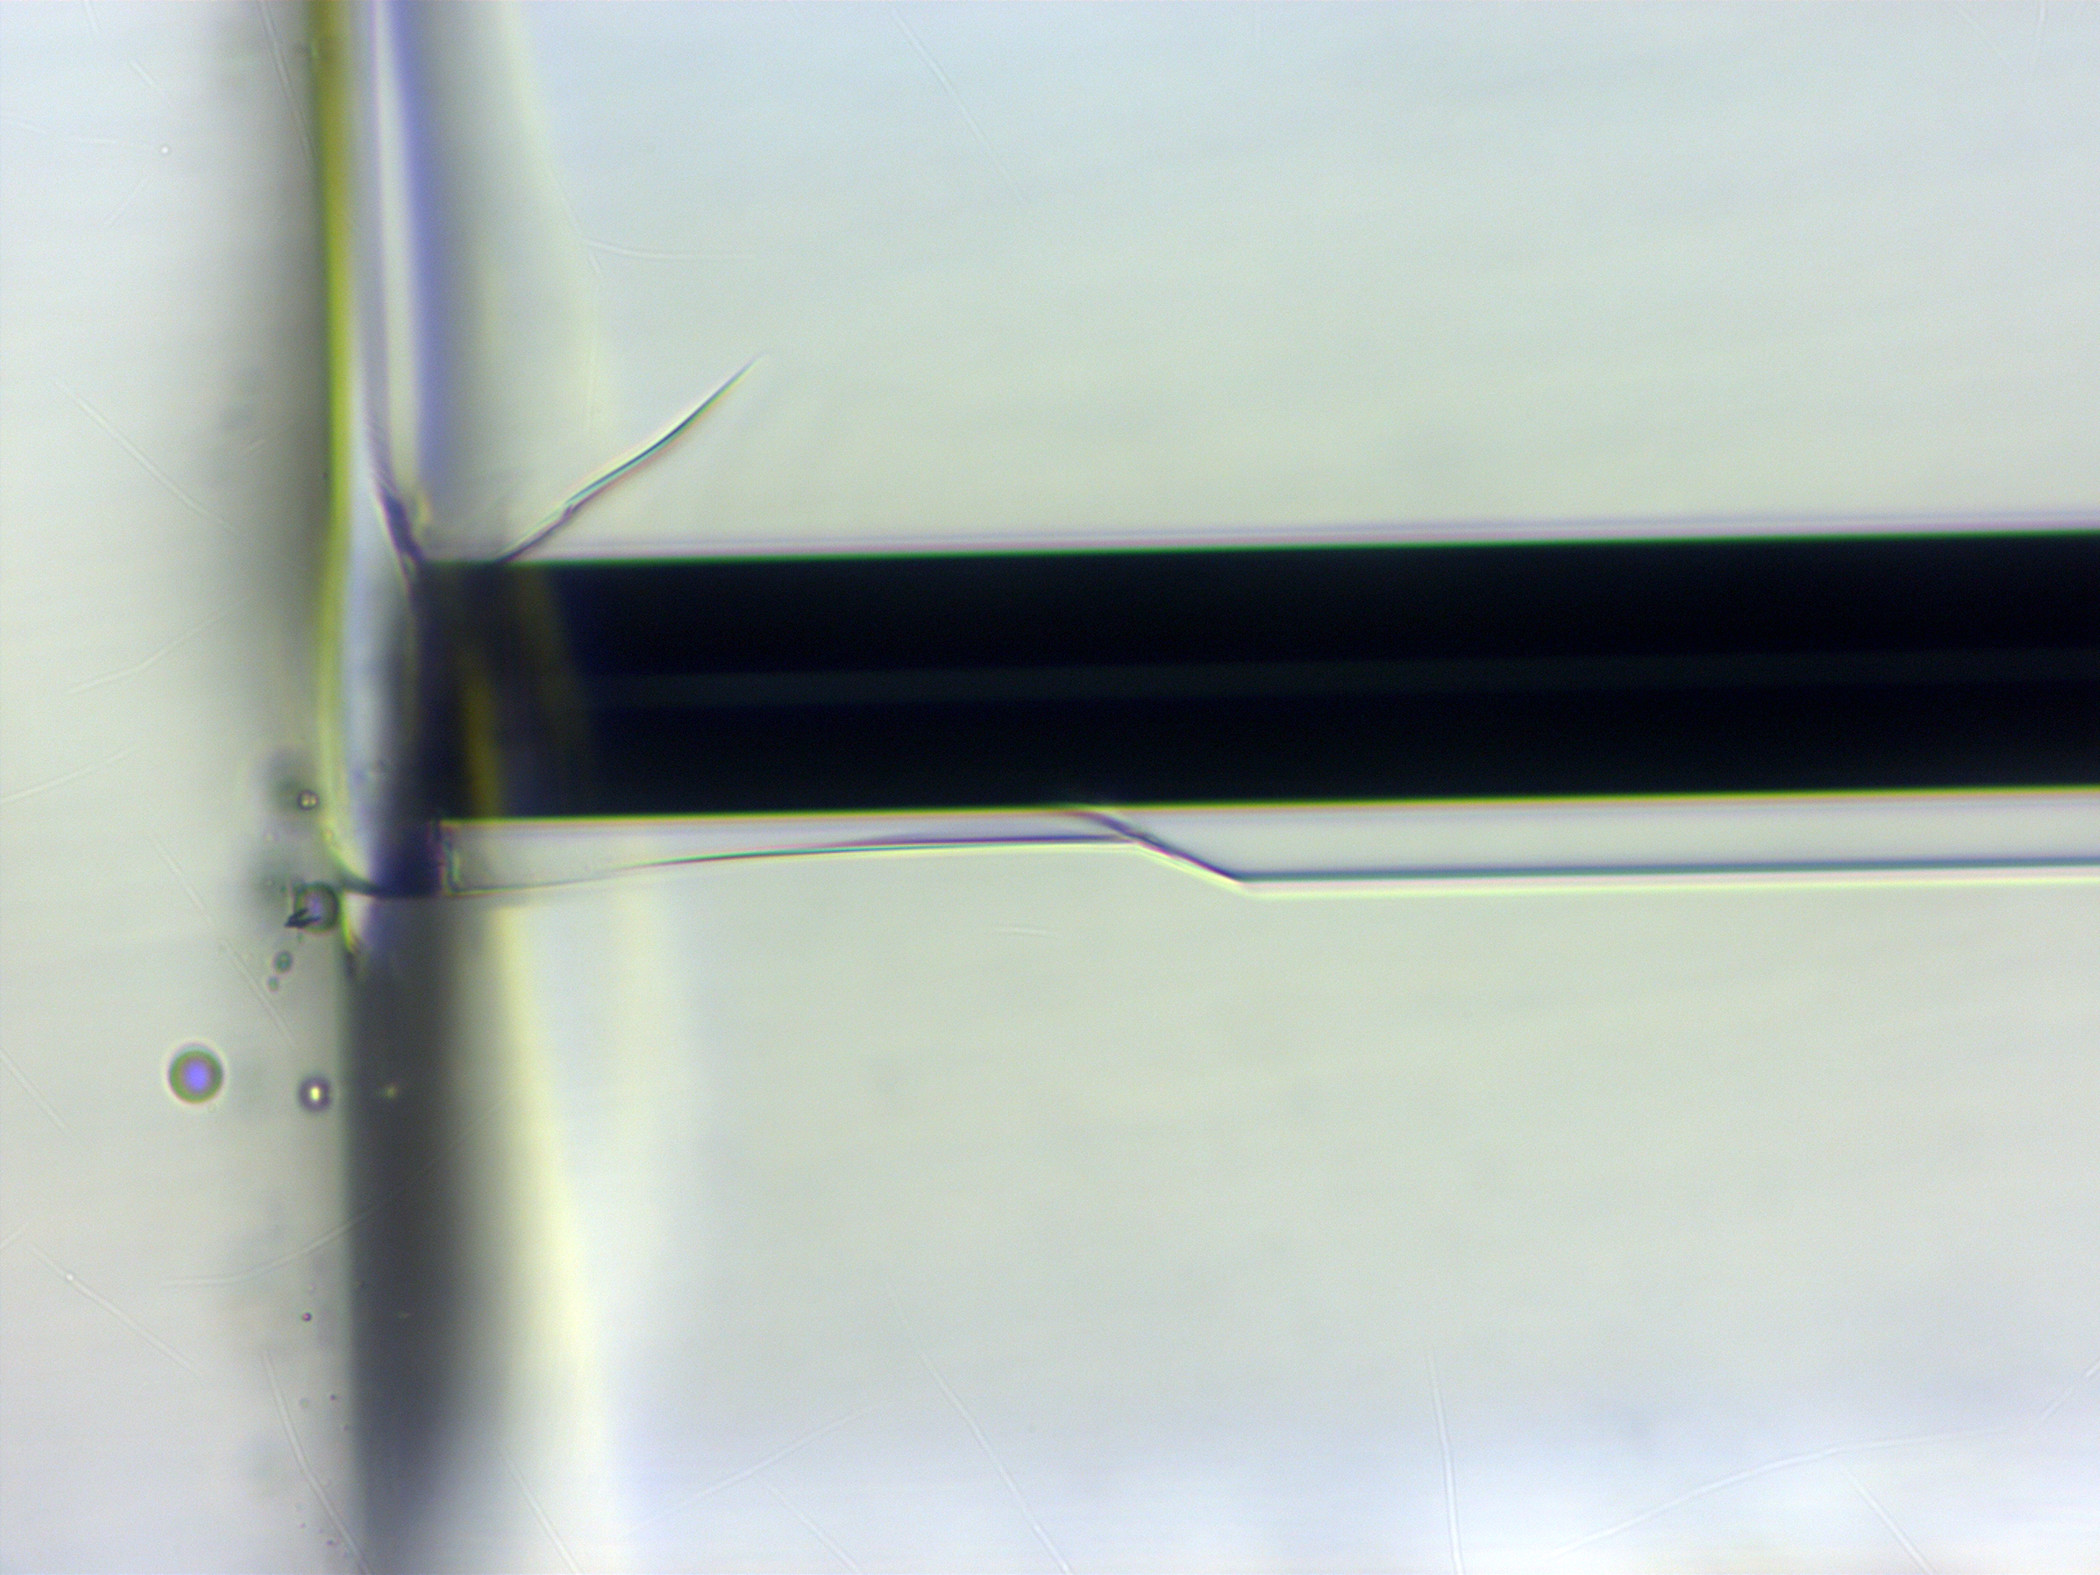
\includegraphics[width=\linewidth]{fig/polishing/parallelcrack2.jpg}
  %\caption{1a}
  \label{fig:sfig2}
\end{subfigure}% %blank line makes figures vertical


 \caption{}
\label{fig:si_sige}
\end{figure}
\FloatBarrier
\subsection{oven anneal}
\begin{figure}[h]
 %h here H requires float, exactly here, h! overide latex
\centering
\begin{subfigure}{\textwidth}
  \centering
  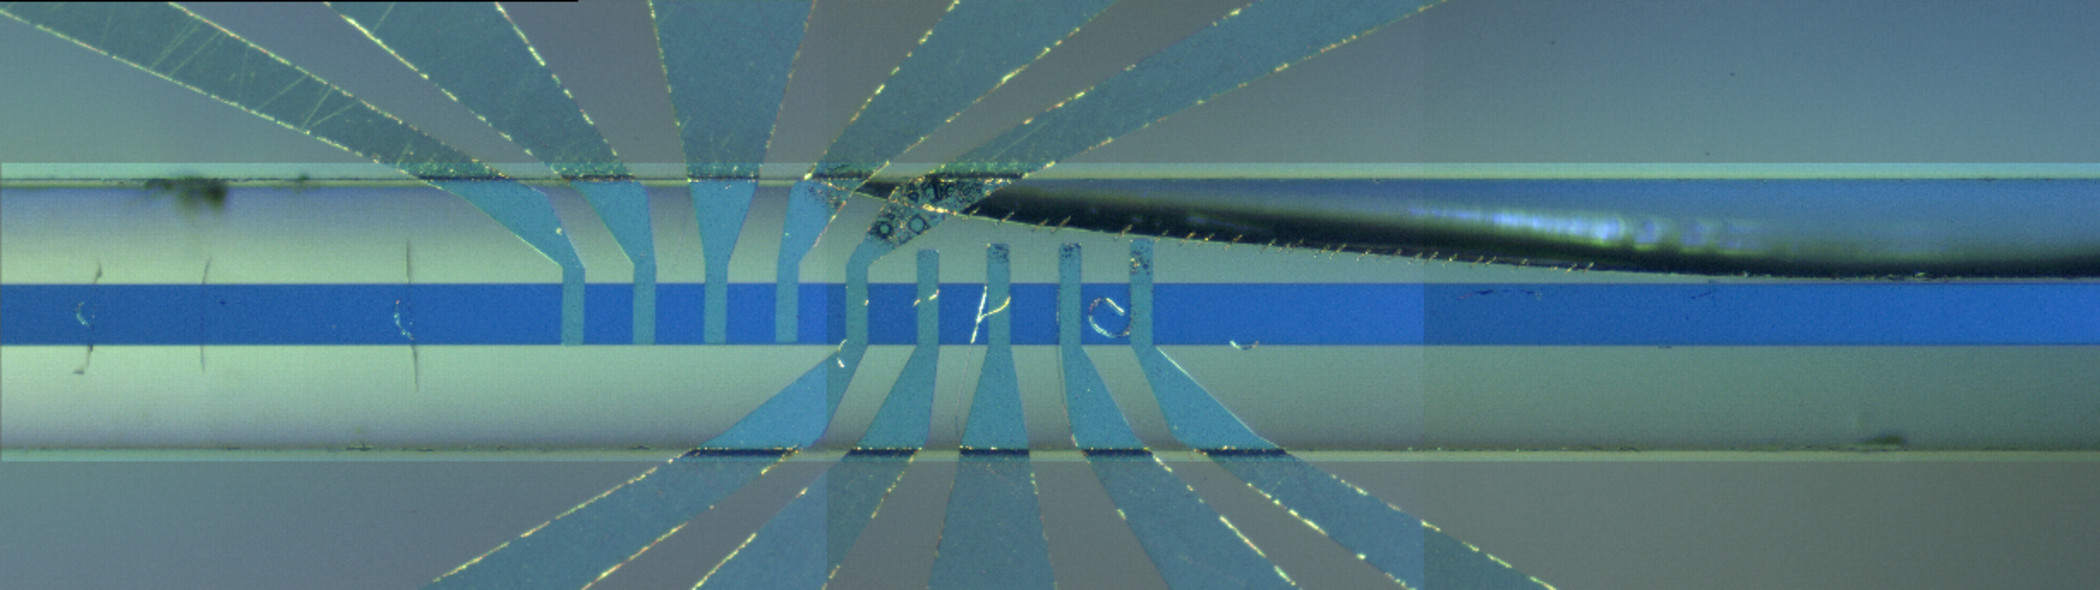
\includegraphics[width=\linewidth]{fig/OA/dd35114_0A--01-1.jpg}
  %\caption{1a}
  \label{fig:sfig1}
\end{subfigure}% %blank line makes figures vertical

\begin{subfigure}{\textwidth}
  \centering
  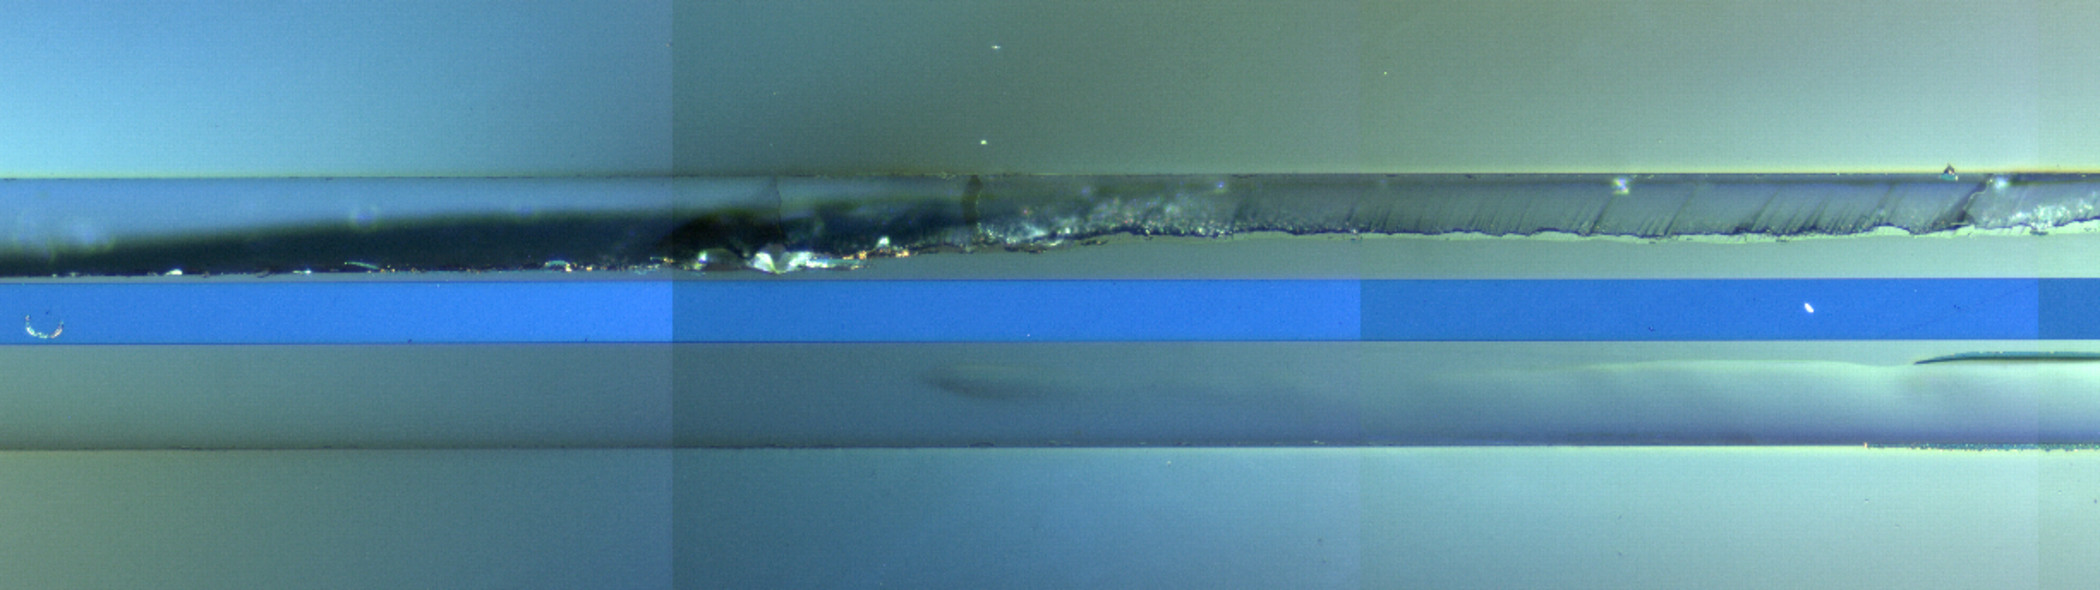
\includegraphics[width=\linewidth]{fig/OA/dd35114_0A--01-2.jpg}
  %\caption{1a}
  \label{fig:sfig2}
\end{subfigure}% %blank line makes figures vertical

\begin{subfigure}{\textwidth}
  \centering
  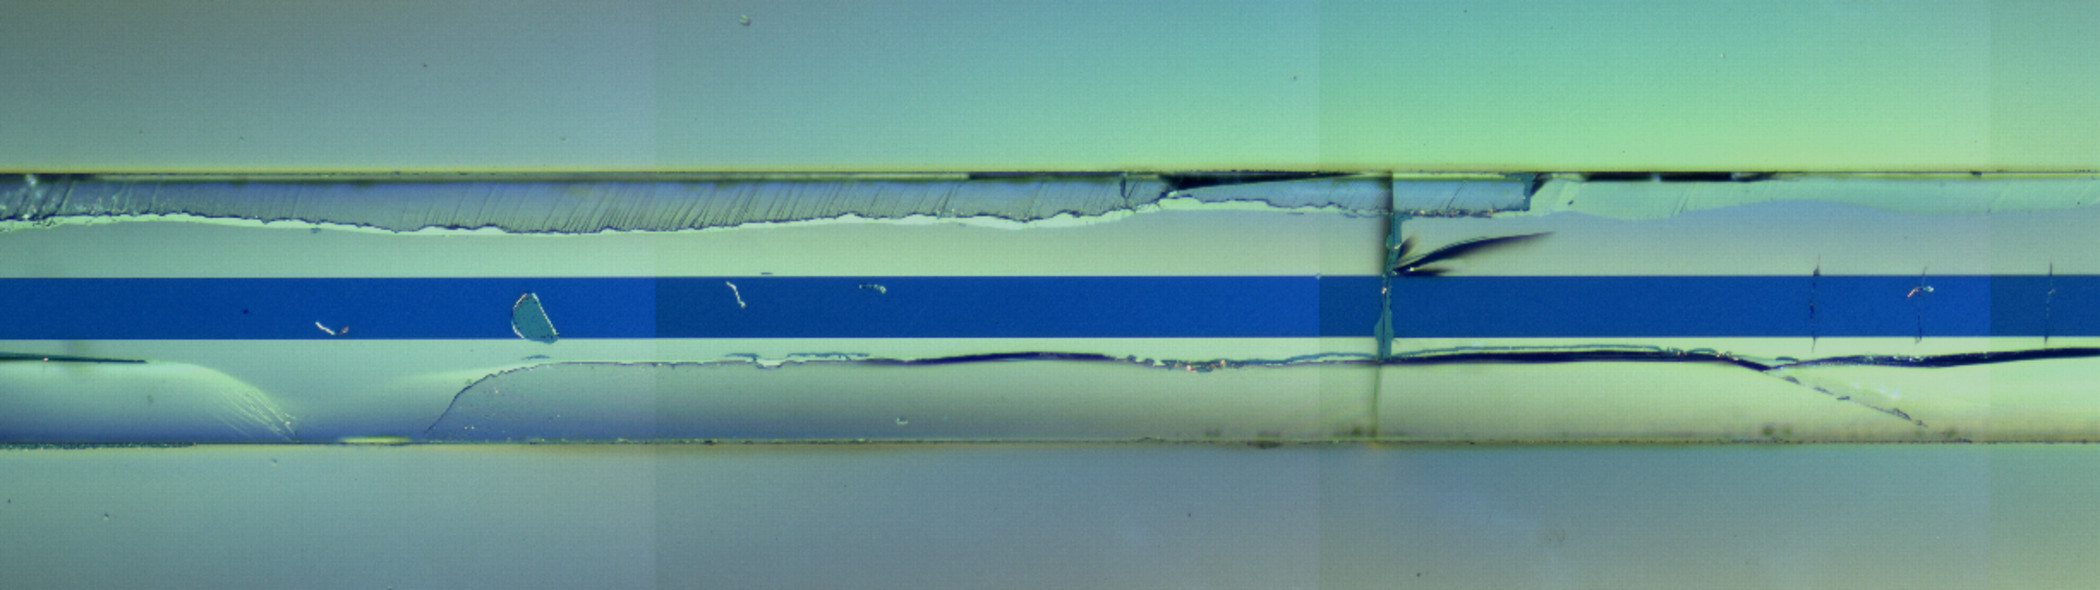
\includegraphics[width=\linewidth]{fig/OA/dd35114_0A--01-3.jpg}
  %\caption{1b}
  \label{fig:sfig3}
\end{subfigure}
\caption{Oven anneal Si fiber with ID dd35114 taken with a reflected light and polorization filter. Large cracks in the cladding, seem to act as a mechanism to relieve stress, as no cracking is observable in the core for these areas. Note due to image stiching, periodic vertical lines appear. }
\label{fig:si_sige}
\end{figure}

\begin{figure}
    \centering
    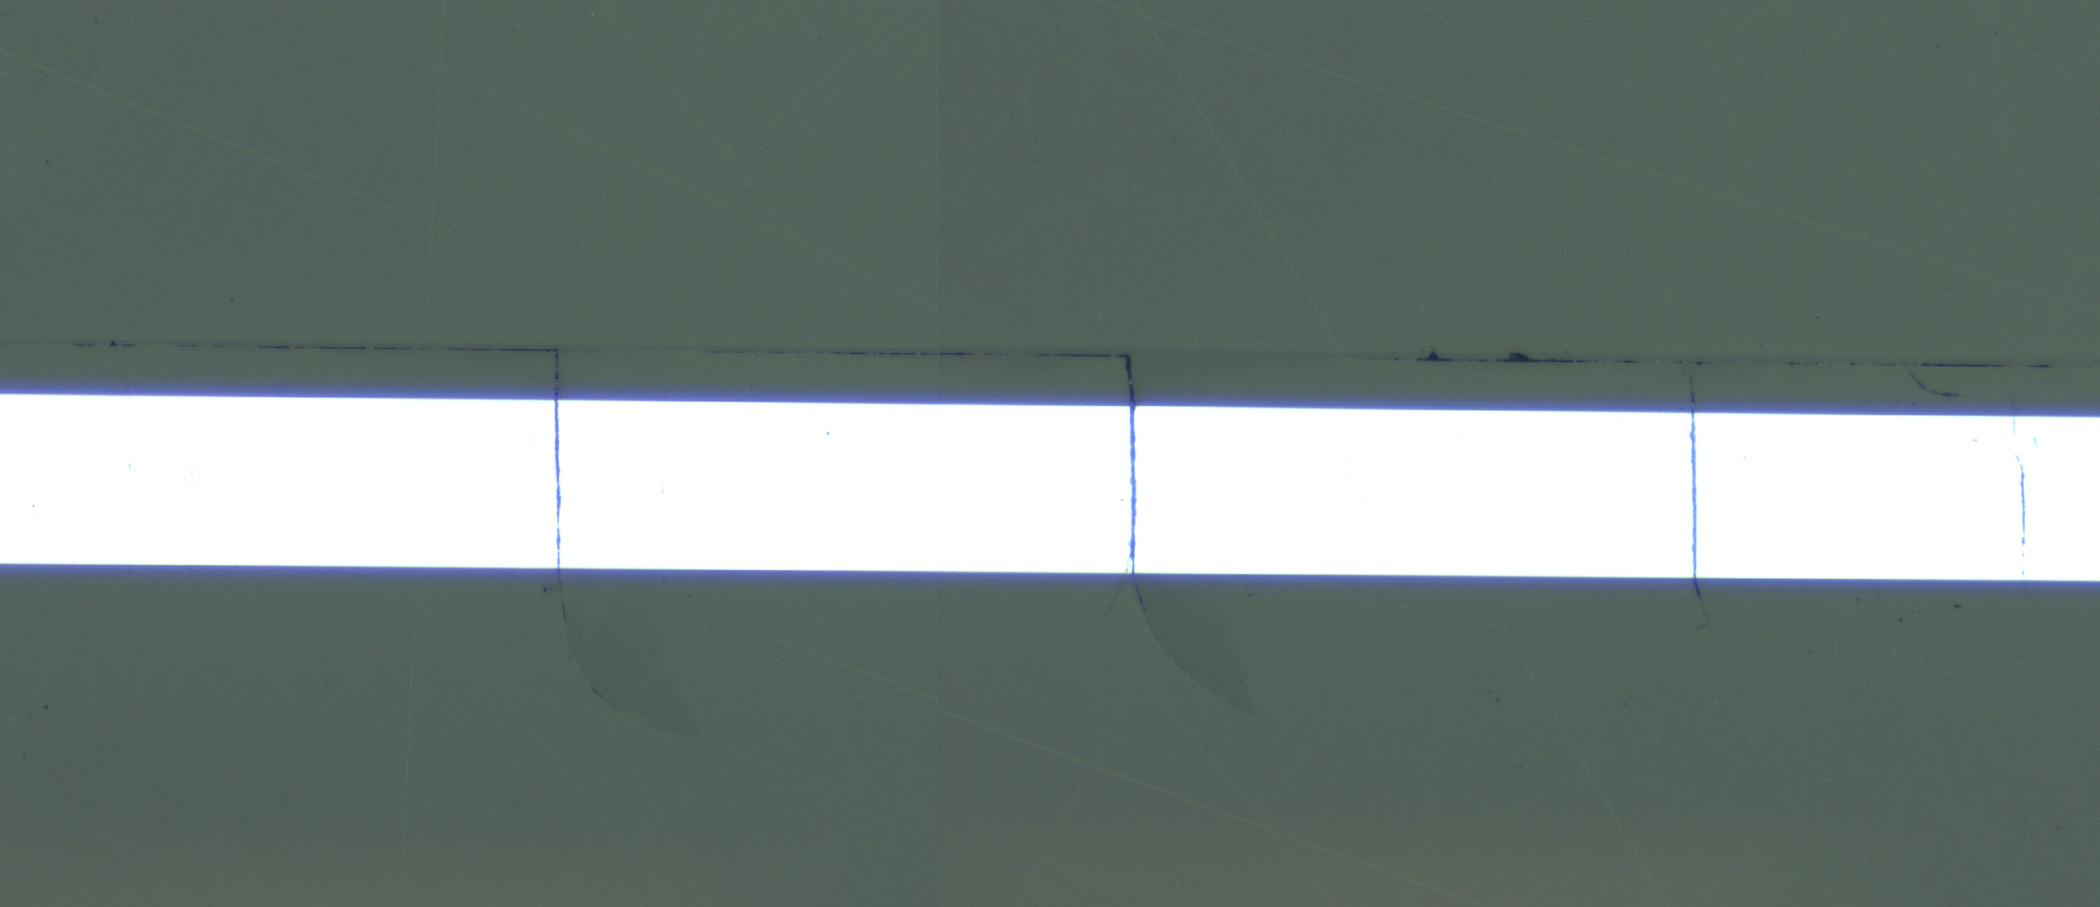
\includegraphics[width=\textwidth]{fig/polishing/dd354114_8.jpg}
    \caption{un annealed DD35114}
    \label{fig:my_label}
\end{figure}



\begin{figure}[h]
 %h here H requires float, exactly here, h! overide latex
\centering
\begin{subfigure}{\textwidth}
  \centering
  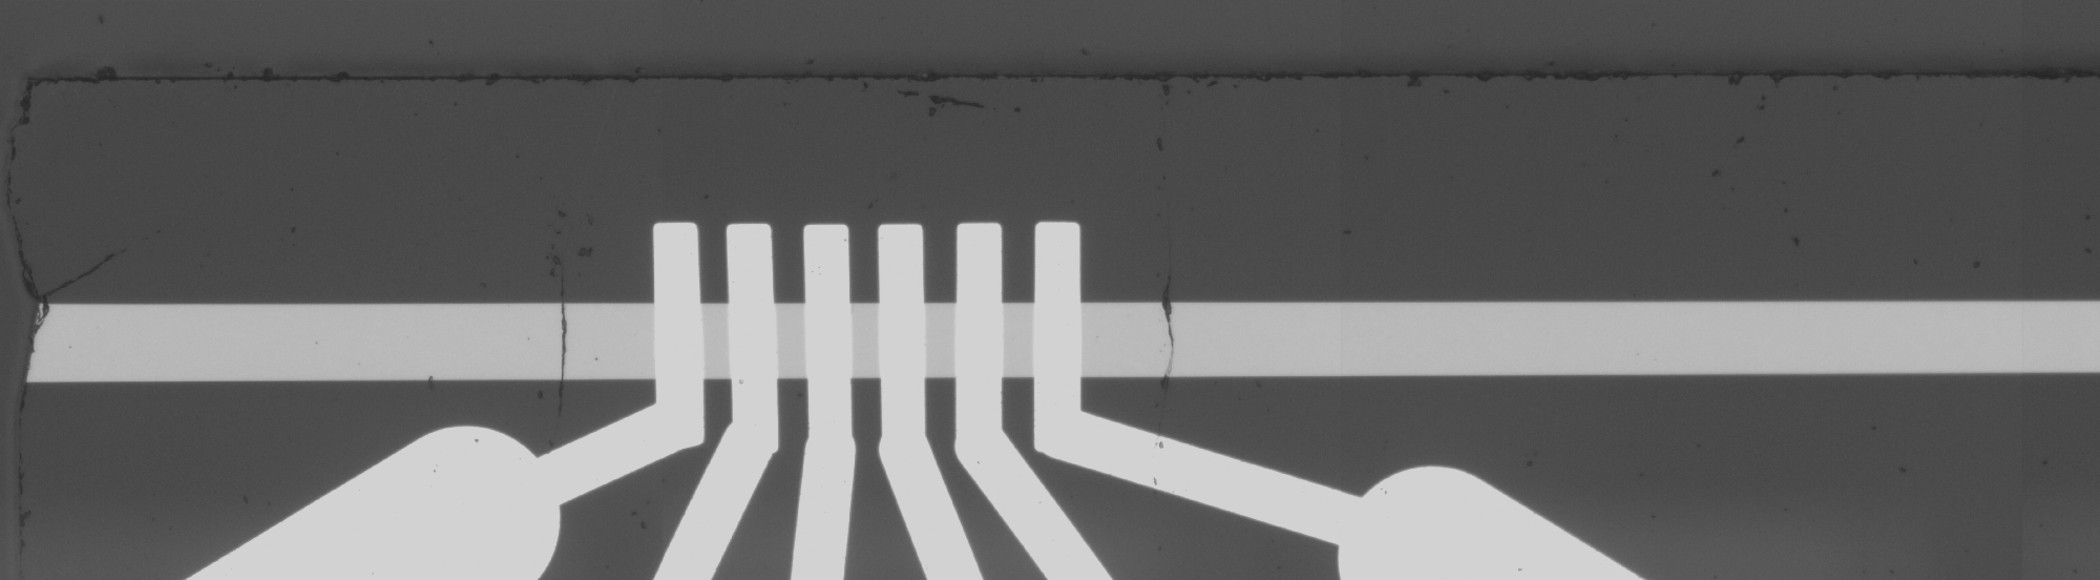
\includegraphics[width=\linewidth]{fig/OA/e944190422_redo-dup1.jpg}
  %\caption{1a}
  \label{fig:sfig1}
\end{subfigure}% %blank line makes figures vertical

\begin{subfigure}{\textwidth}
  \centering
  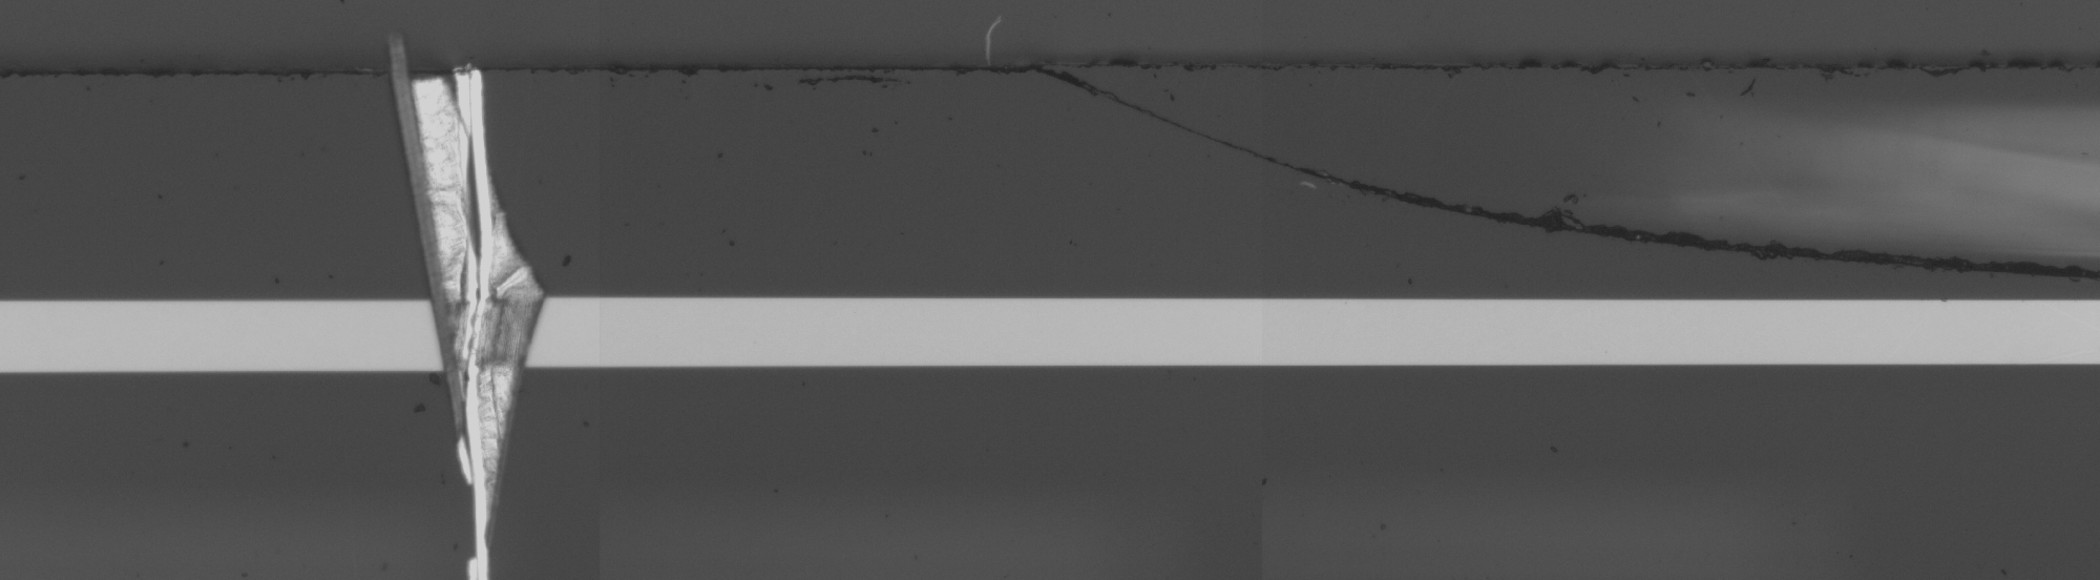
\includegraphics[width=\linewidth]{fig/OA/e944190422_redo-duplicate2.jpg}
  %\caption{1a}
  \label{fig:sfig2}
\end{subfigure}% %blank line makes figures vertical

\caption{Da13118 Annealed }
\label{fig:si_sige}
\end{figure}


\begin{figure}[h]
    \centering
    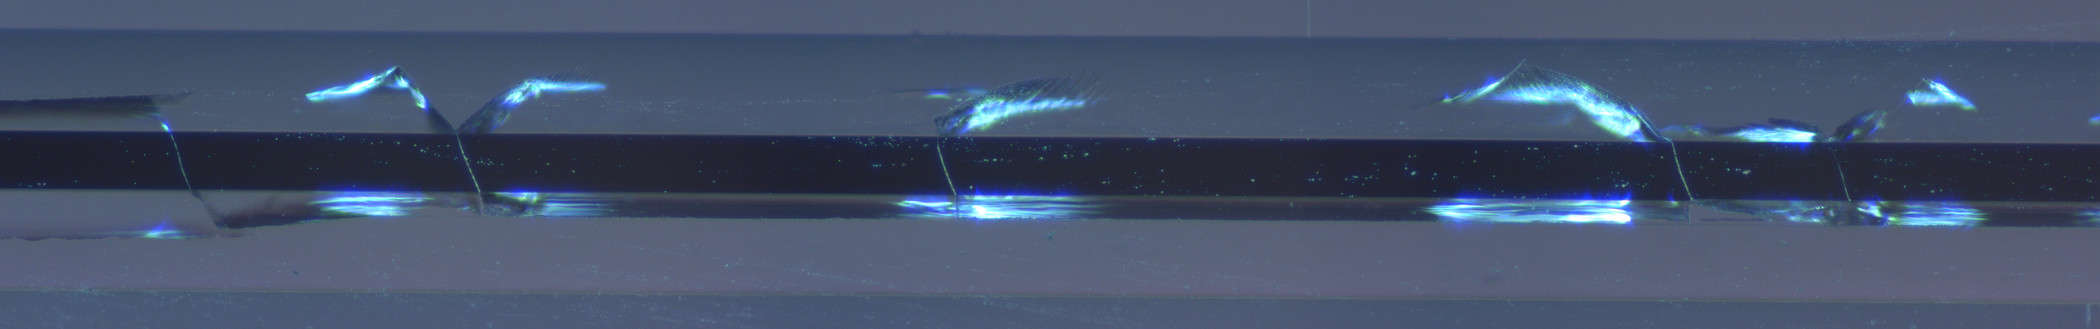
\includegraphics[width=\textwidth]{fig/polishing/e944.jpg}
    \caption{un annealed DA13118}
    \label{fig:my_label}
\end{figure}
\FloatBarrier
\subsection{Maskless Lithography}
\subsection{Permanent Resist Underlayer}
Discussion of deposition results and electrical measurements. 
conclusion: successful but need better deposition method, i.e new e-beam with sample tilt. Better sample cleaing after lithography steps and optimization of the recipe, especially exposure and development time for clean patterns. mr-dwl resist likely leaving some contamination.

\begin{figure}[h!]
 %h here H requires float, exactly here, h! overide latex
\centering
\begin{subfigure}{\textwidth}
  \centering
  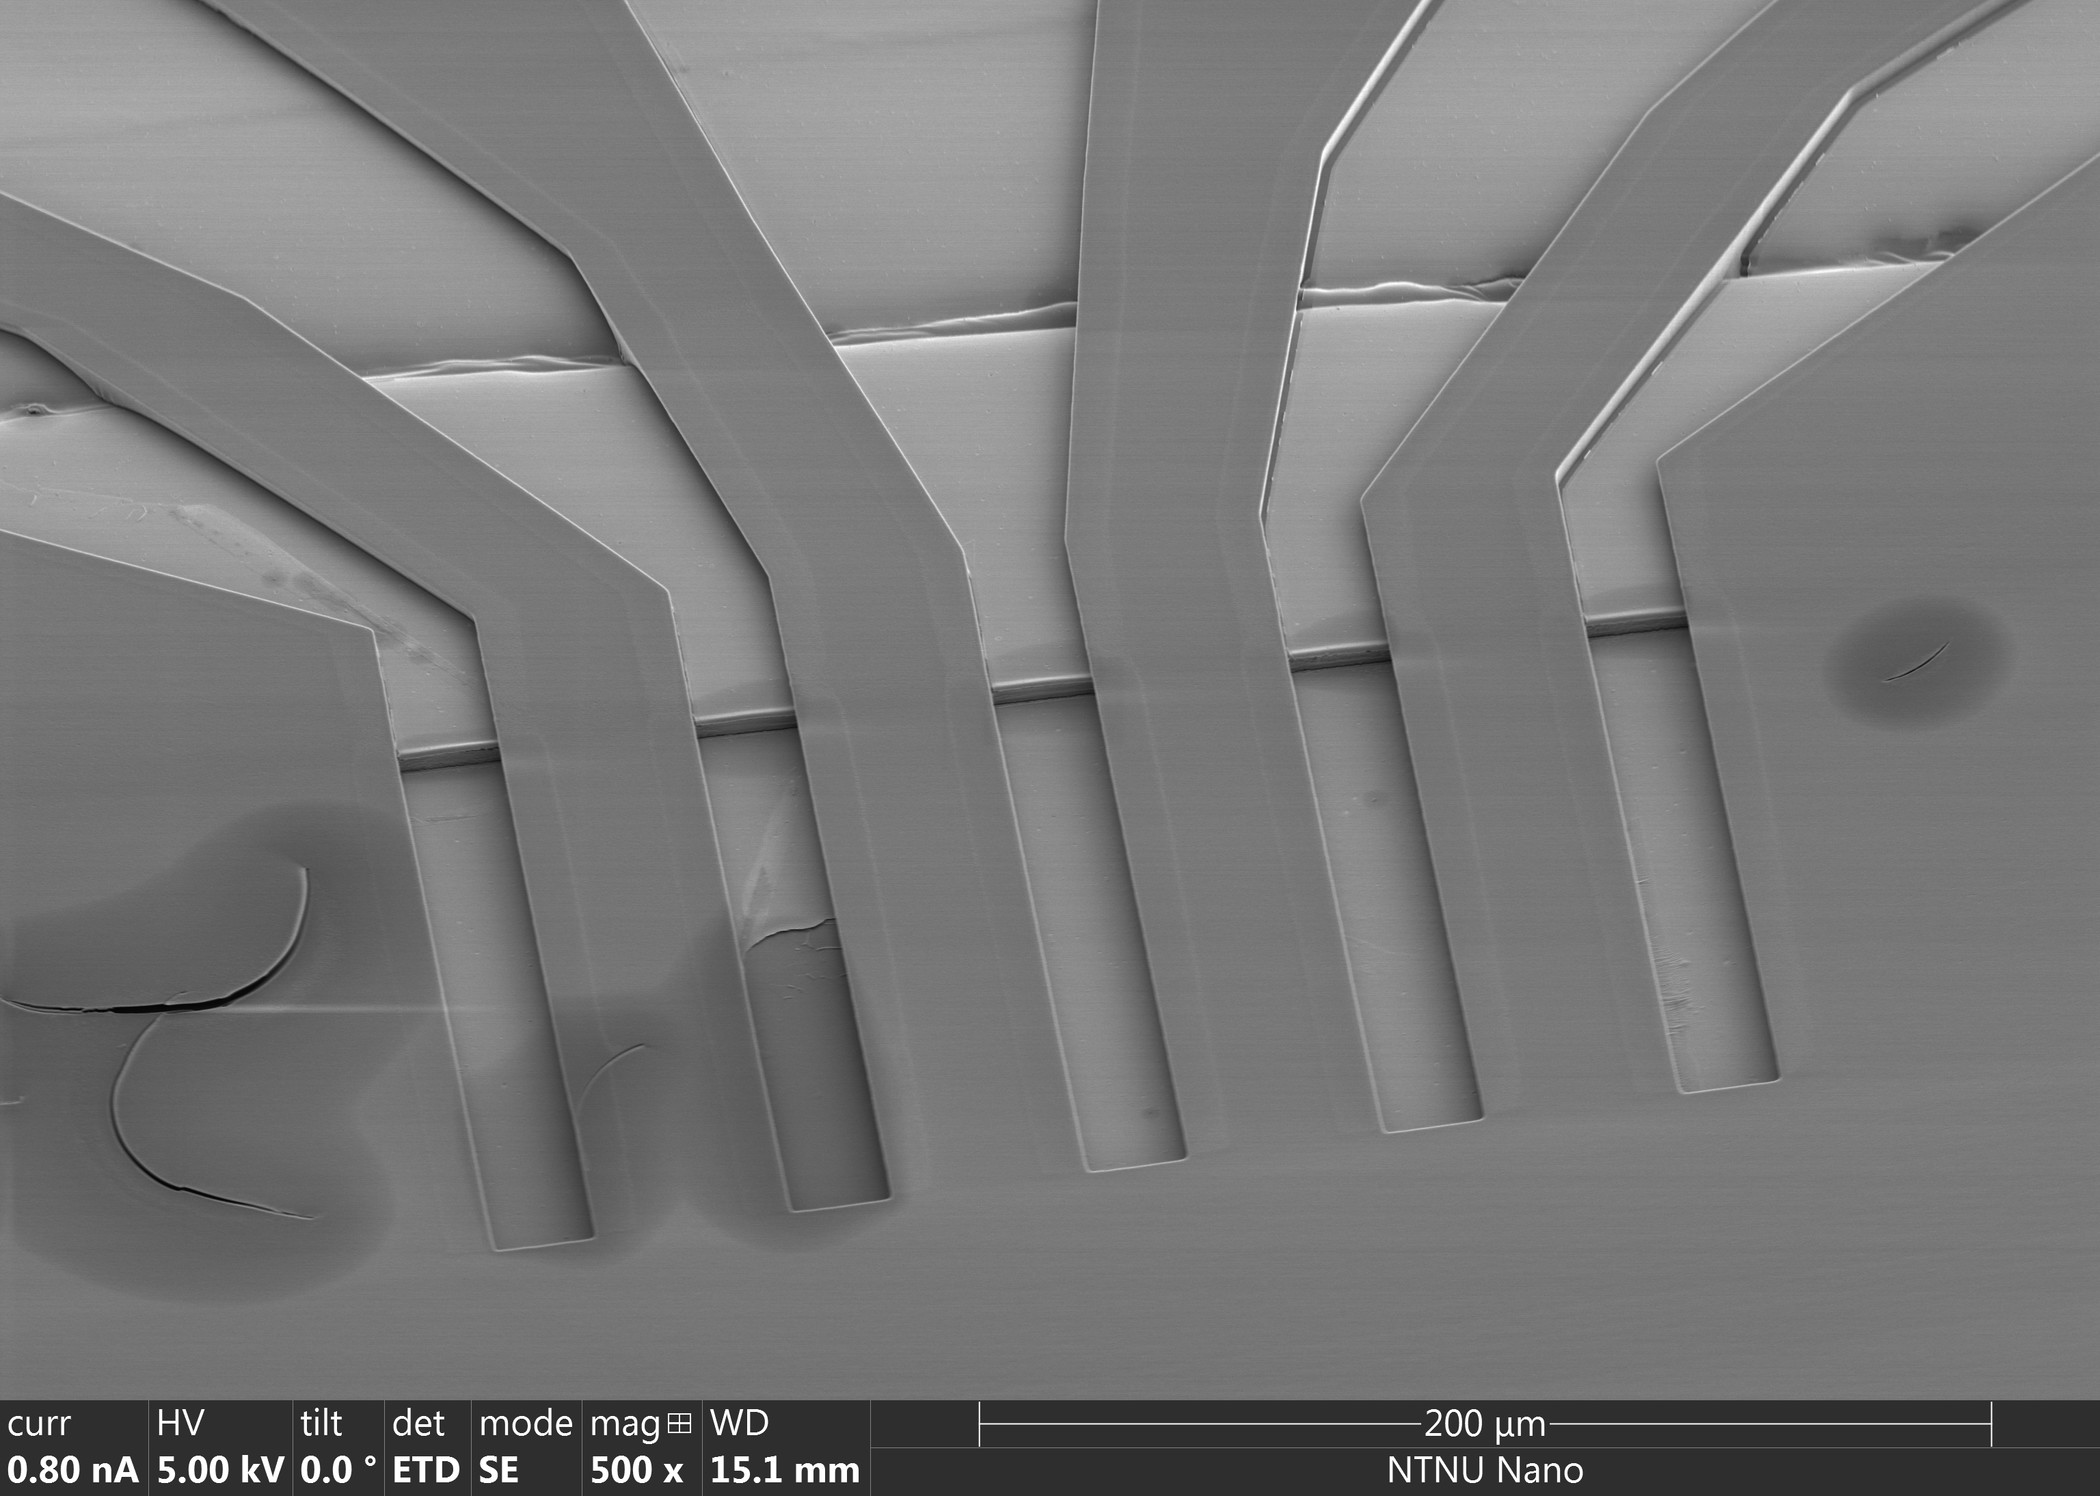
\includegraphics[width=\linewidth]{fig/mr-DWL/mb_25_overview_002.jpg}
  %\caption{1a}
  \label{fig:sfig1}
\end{subfigure}% %blank line makes figures vertical

\begin{subfigure}{\textwidth}
  \centering
  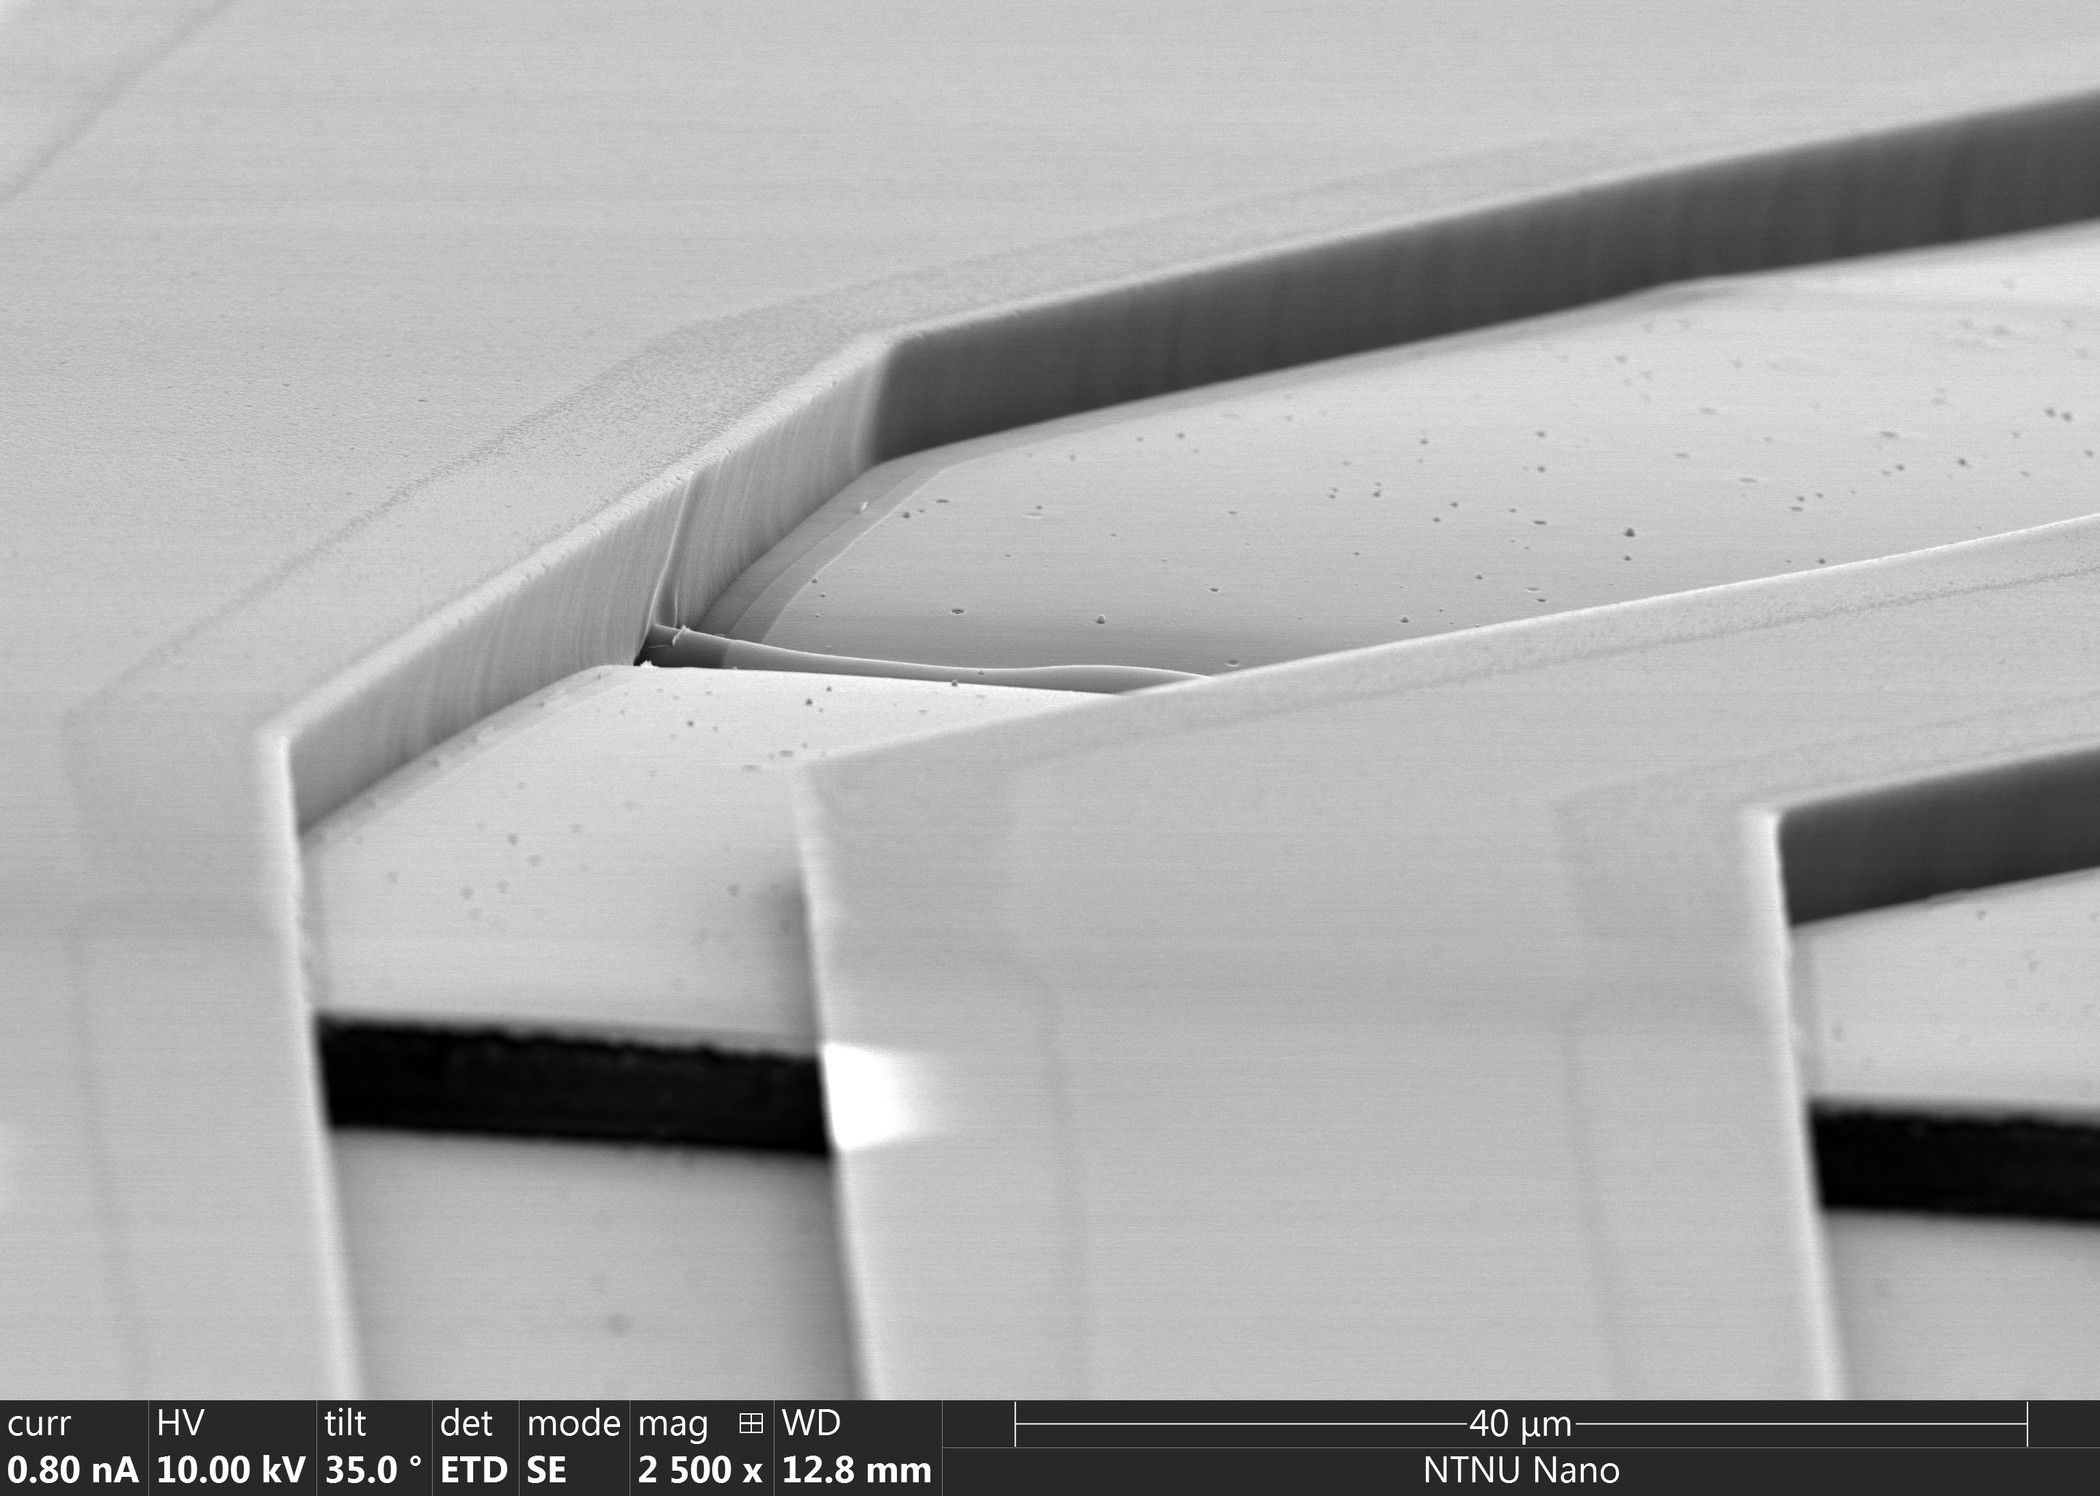
\includegraphics[width=\linewidth]{fig/mr-DWL/mb_25_step_004.jpg}
  %\caption{1a}
  \label{fig:sfig2}
\end{subfigure}% %blank line makes figures vertical

\caption{}
\label{fig:si_sige}
\end{figure}


\begin{figure}[h!]
 %h here H requires float, exactly here, h! overide latex
\centering
\begin{subfigure}{\textwidth}
  \centering
  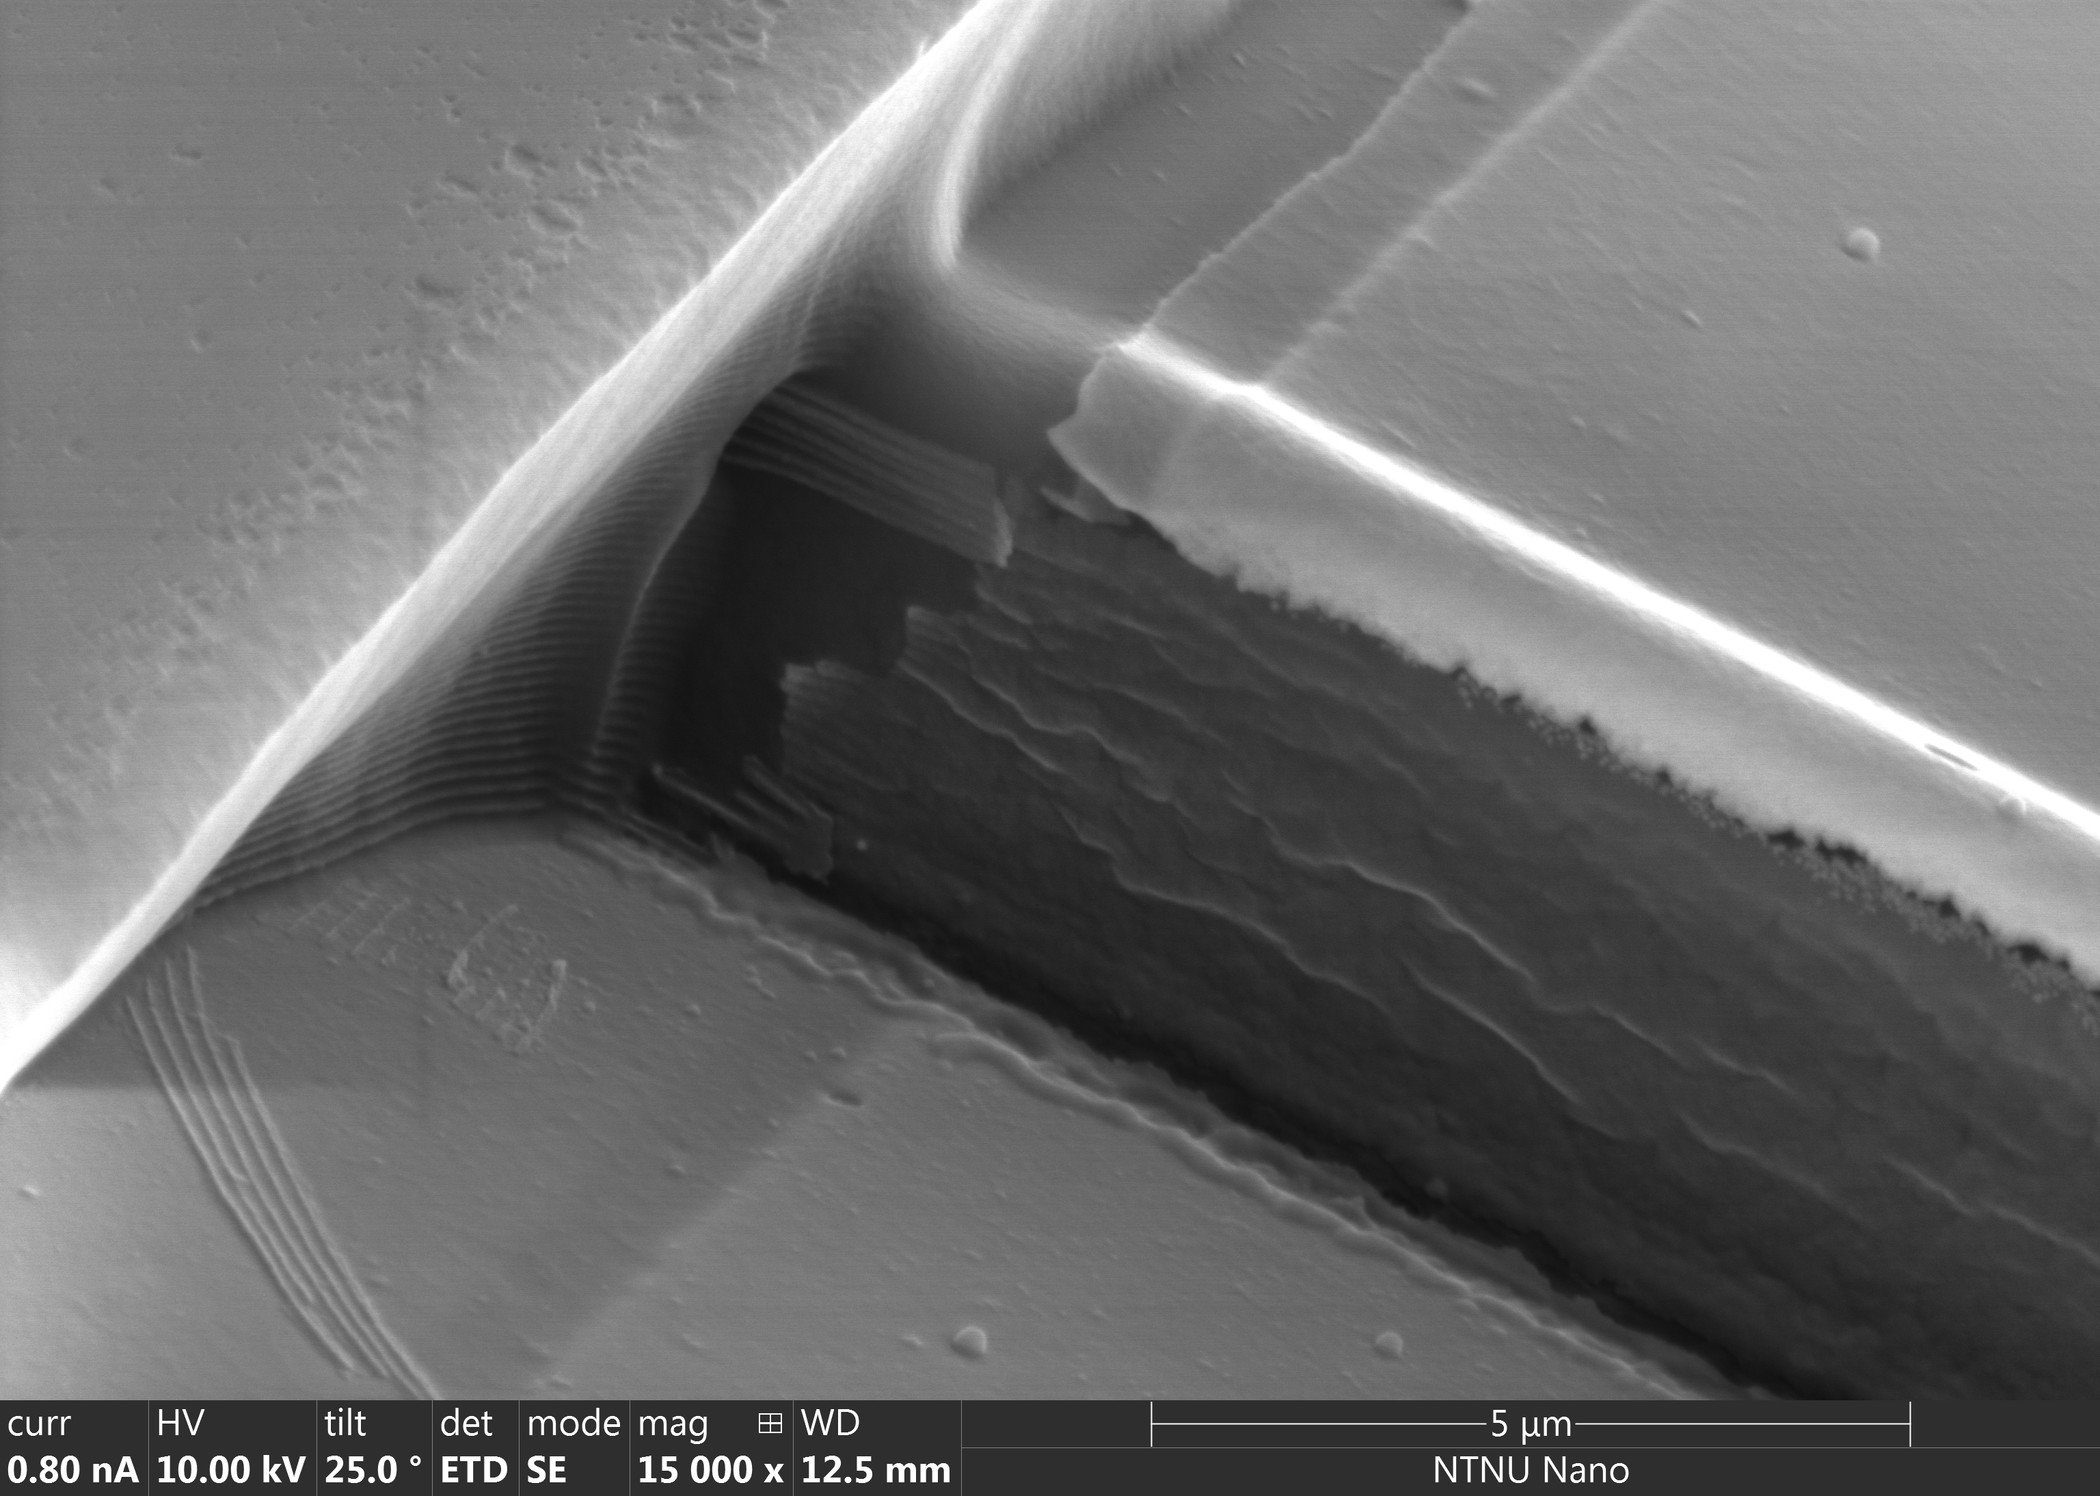
\includegraphics[width=\linewidth]{fig/mr-DWL/mb_25_step_close1.jpg}
  %\caption{1a}
  \label{fig:sfig1}
\end{subfigure}% %blank line makes figures vertical


\caption{}
\label{fig:si_sige}
\end{figure}


\begin{figure}[h!]
    \centering
    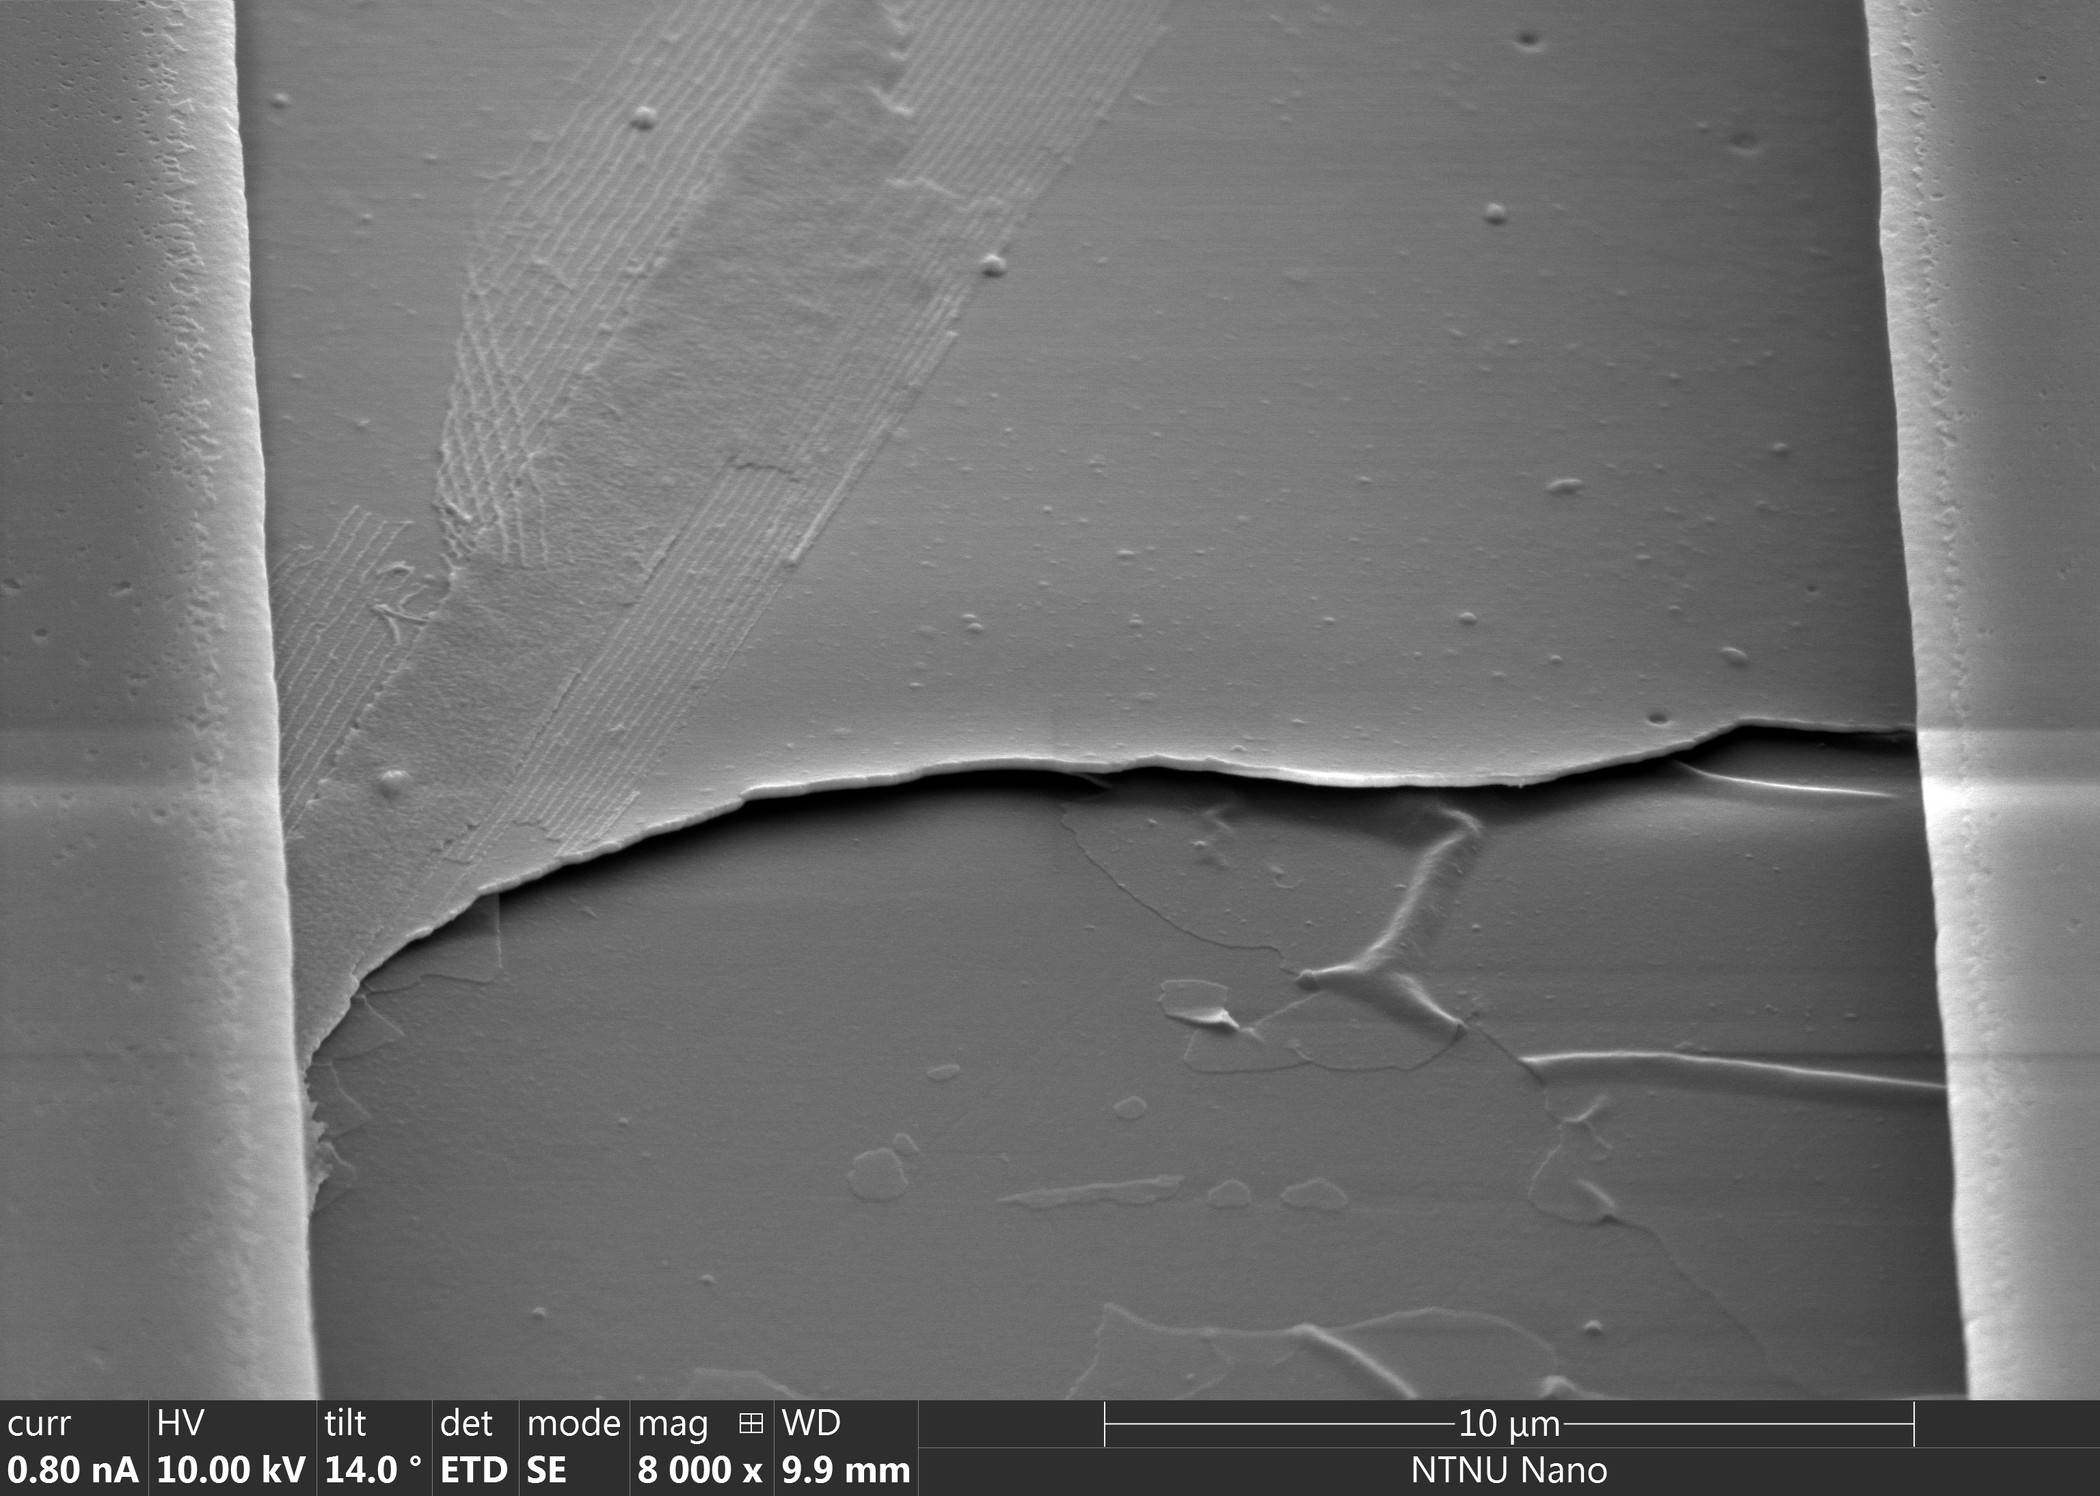
\includegraphics[width=\textwidth]{fig/mr-DWL/mb_25_step_002.jpg}
    \caption{Caption}
    \label{fig:my_label}
\end{figure}


\FloatBarrier




\cleardoublepage
